\chapter{Appendix F: Extra Plots and Figures}
\label{AppendixF}

\section{Sobol Analysis With Washin and Washout}
\label{sec:AppendixF:sobol_analysis_with_washin_and_washout}
\subsection{Final Value Analysis}
\subsubsection{Resources}
Despite the resource consumption rate directly depending on $e, v$, and $K$, the parameters had very little influence on the final value, as evidenced by the $ST$ and $S1$ bars being near 0. 
The washin and washout values mainly drove the resource population. 
The peak resources are driven entirely by the washin rate. 
There were few interactions between two or more parameters. 

\subsubsection{Phages}
The most important factor for the final phage value is $r$, followed by $\beta$ and $\omega^o$. 
The other parameters had little to no effect on the final phage value. 

\subsubsection{Total Bacteria}
The sum of uninfected and infected bacteria depended heavily on higher-order interactions as $ST_i \gg S1_i$. 
Although not shown, the bar plots for the total bacteria resembled those of the bar plots for the uninfected bacteria, and were less than those of the infected bacteria. 

\subsection{Peak Value and Time of peak}
To create the custom Sobol analyses, the peak value and the time at the peak of the population is measured and analyzed. 
The peak is defined as the point at which the population reaches 95\% of its absolute maximum value. 
The time at peak is measured at the point in time that the population reaches 95\% of the maximum value. 
This removes unintended side effects of the simulation. 
For populations that are only increasing in value, this prevents the measured peak from clustering at the end of the simulation, thereby skewing the data. 
As the peak is defined at 95\% of the absolute maximum value, populations that experience a faster increase in population count at the end will have a time value closer to the end of the simulation. 
For populations that reach a plateau, the 95\% rule will push the time of peak towards the beginning of the simulation while still “respecting” the absolute final value since $95\% \approx 100\%$. 
The 95\% rule can fail under certain situations, such as when there is cyclic behavior. 
See \Cref{sec:appendixF:why_95} for a more detailed explanation on why the 95\% rule is used. 

The results of the Sobol peak and time at peak analyses can be seen in \Cref{fig:created:Sobol_peak} and \Cref{fig:created:Sobol_peak_time}. 
Although some bars between the final, peak, and time at peak values are the same, others differ. 
However, overall, similar values can be seen across the final, peak, and time at peak analyses. 
The peak infected values are more certain compared to the final infected values, which could be due to the 95\% rule removing some of the noise of the simulation. 
The time at peak values have less error compared to the final and peak values. 
This is due to the restricted range of values. The time at peak value can only fall somewhere between 0 and 15, which corresponds to the start and end values of the simulation, respectively. 
The final and peak values can fall anywhere between 0 and any value, depending on the IC and how high the population can rise, as well as how fast the population can fall, \textit{if} the population count falls. 

\begin{figure}[ht!]
    \centering
    \begin{subfigure}{0.32\linewidth}
        \centering
        \captionsetup{width=1\linewidth}
        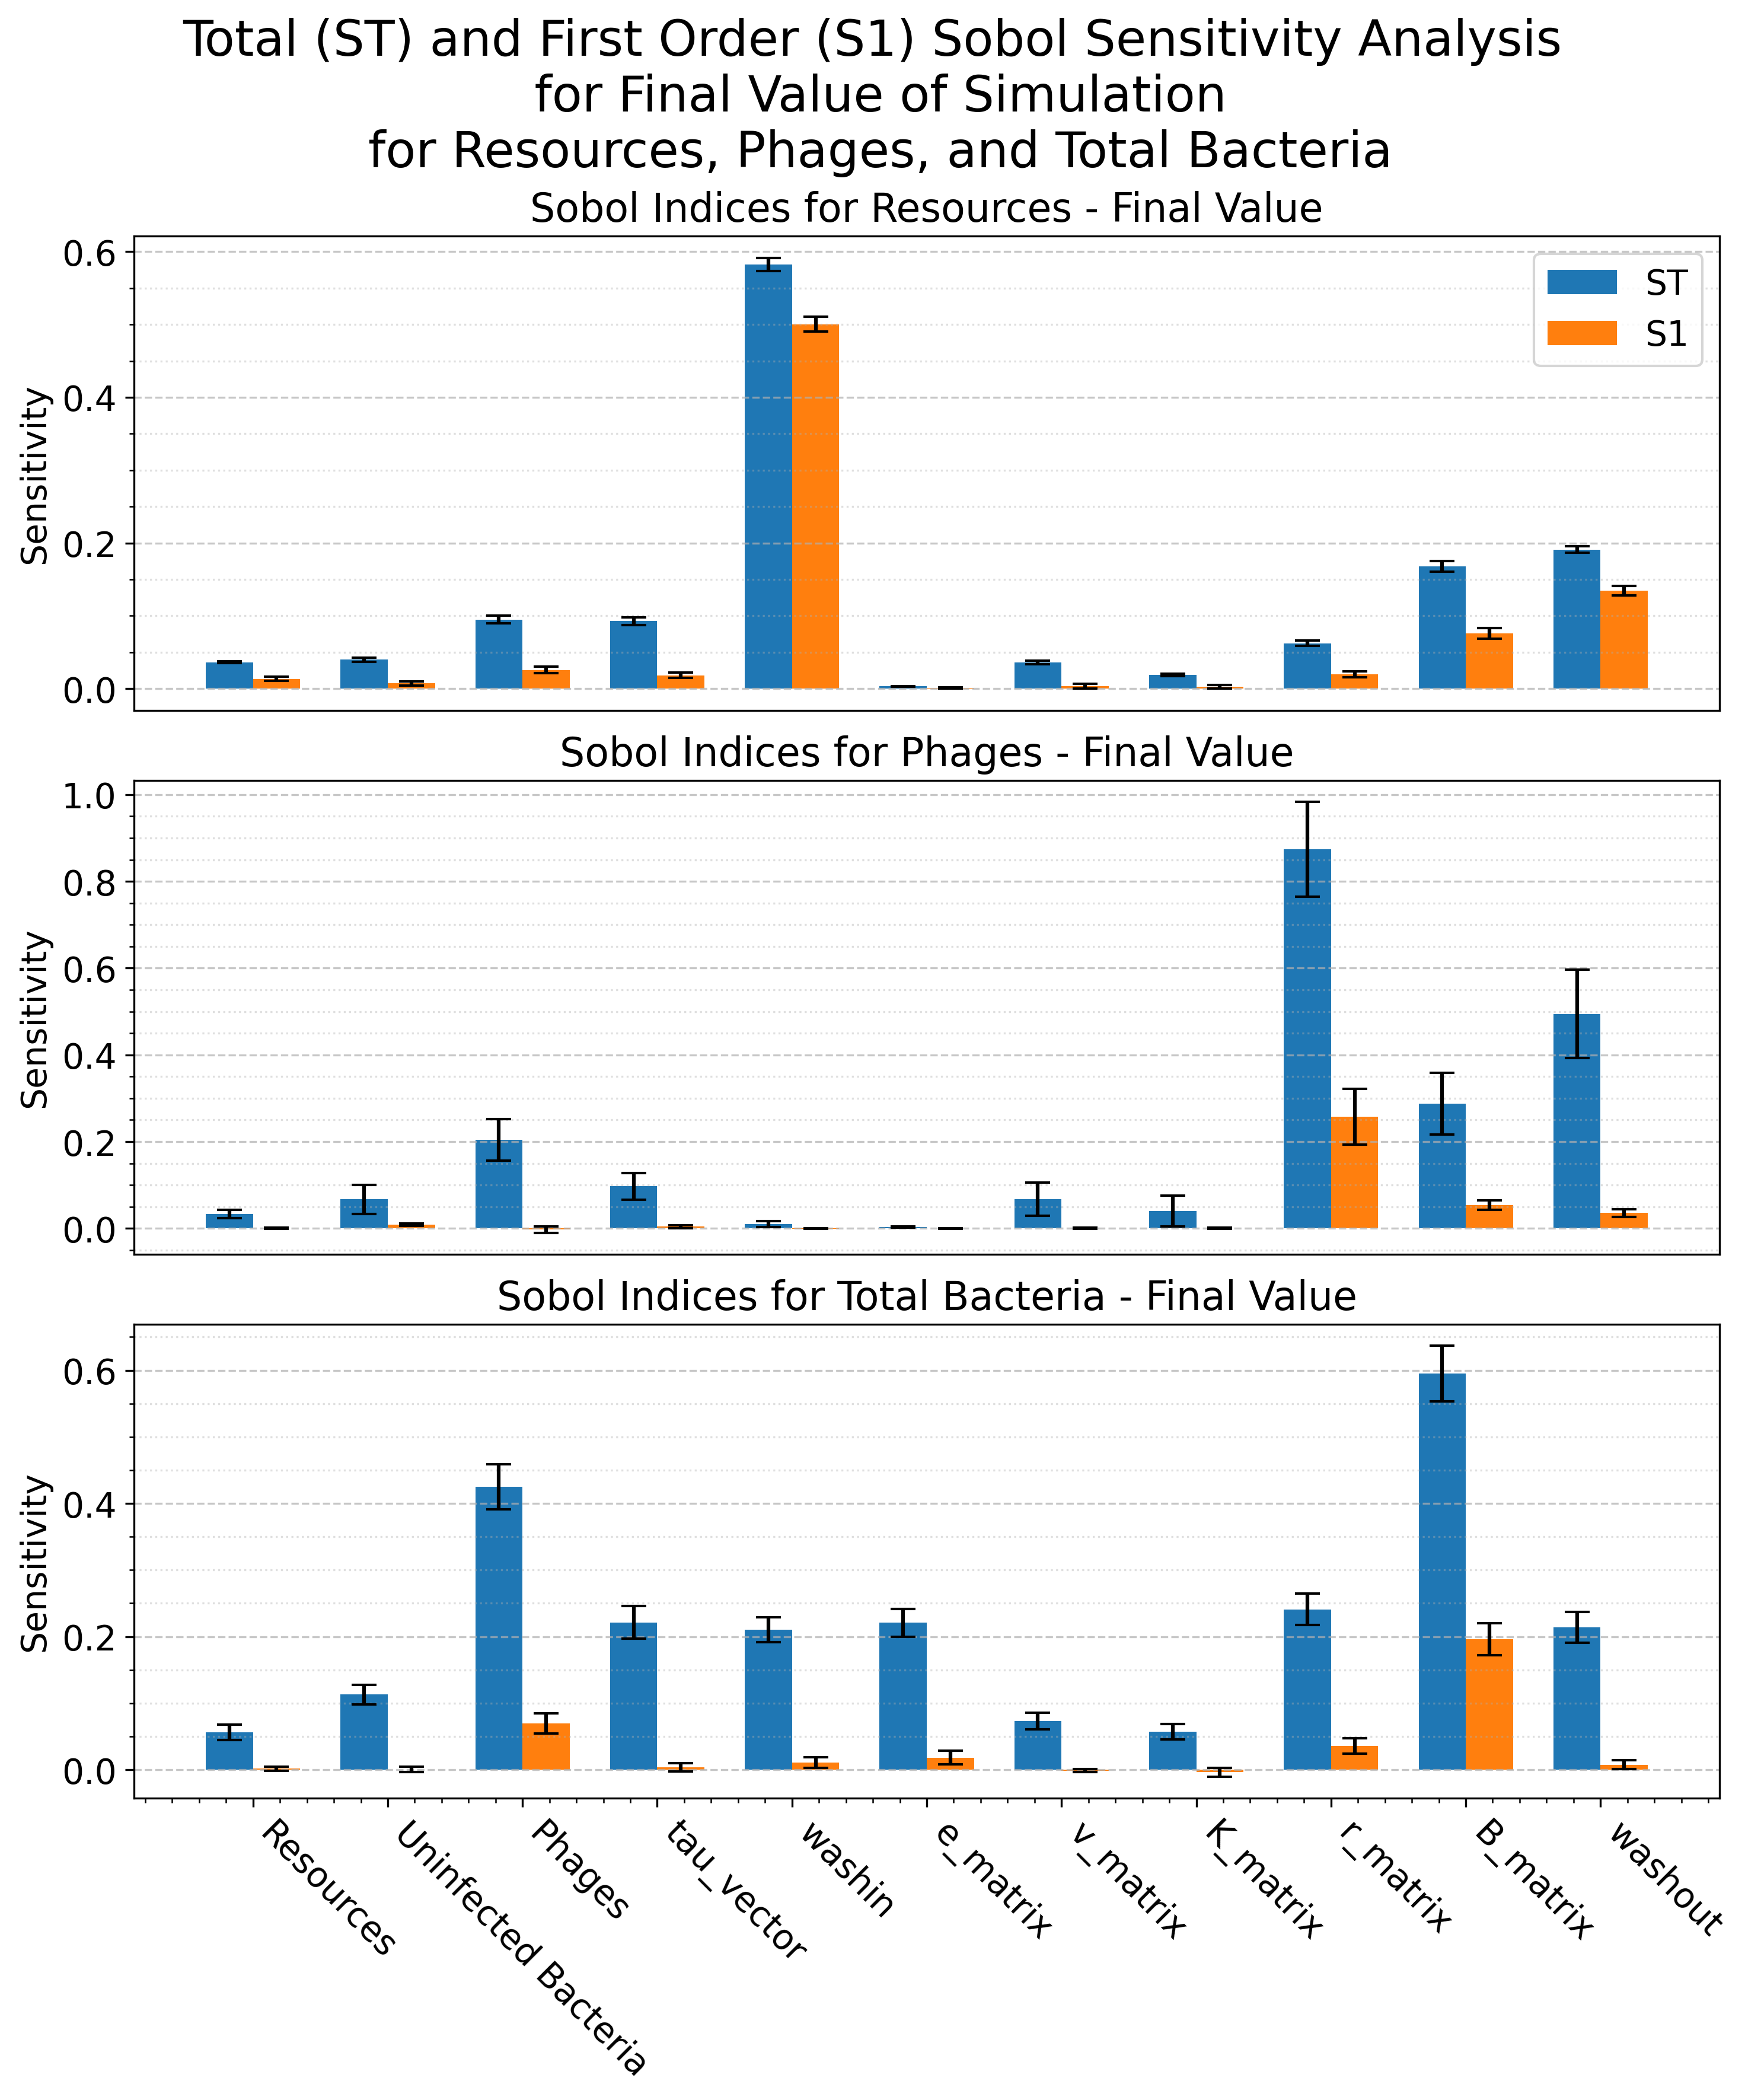
\includegraphics[width=\linewidth]{Plots/Created/SOBOL/SOBOL_analysis_1749149674_Final.png}
        \caption{
            Final population value. 
        }
        \label{fig:created:Sobol_final}
    \end{subfigure}
    \hfill
    \begin{subfigure}{0.32\linewidth}
        \centering
        \captionsetup{width=1\linewidth}
        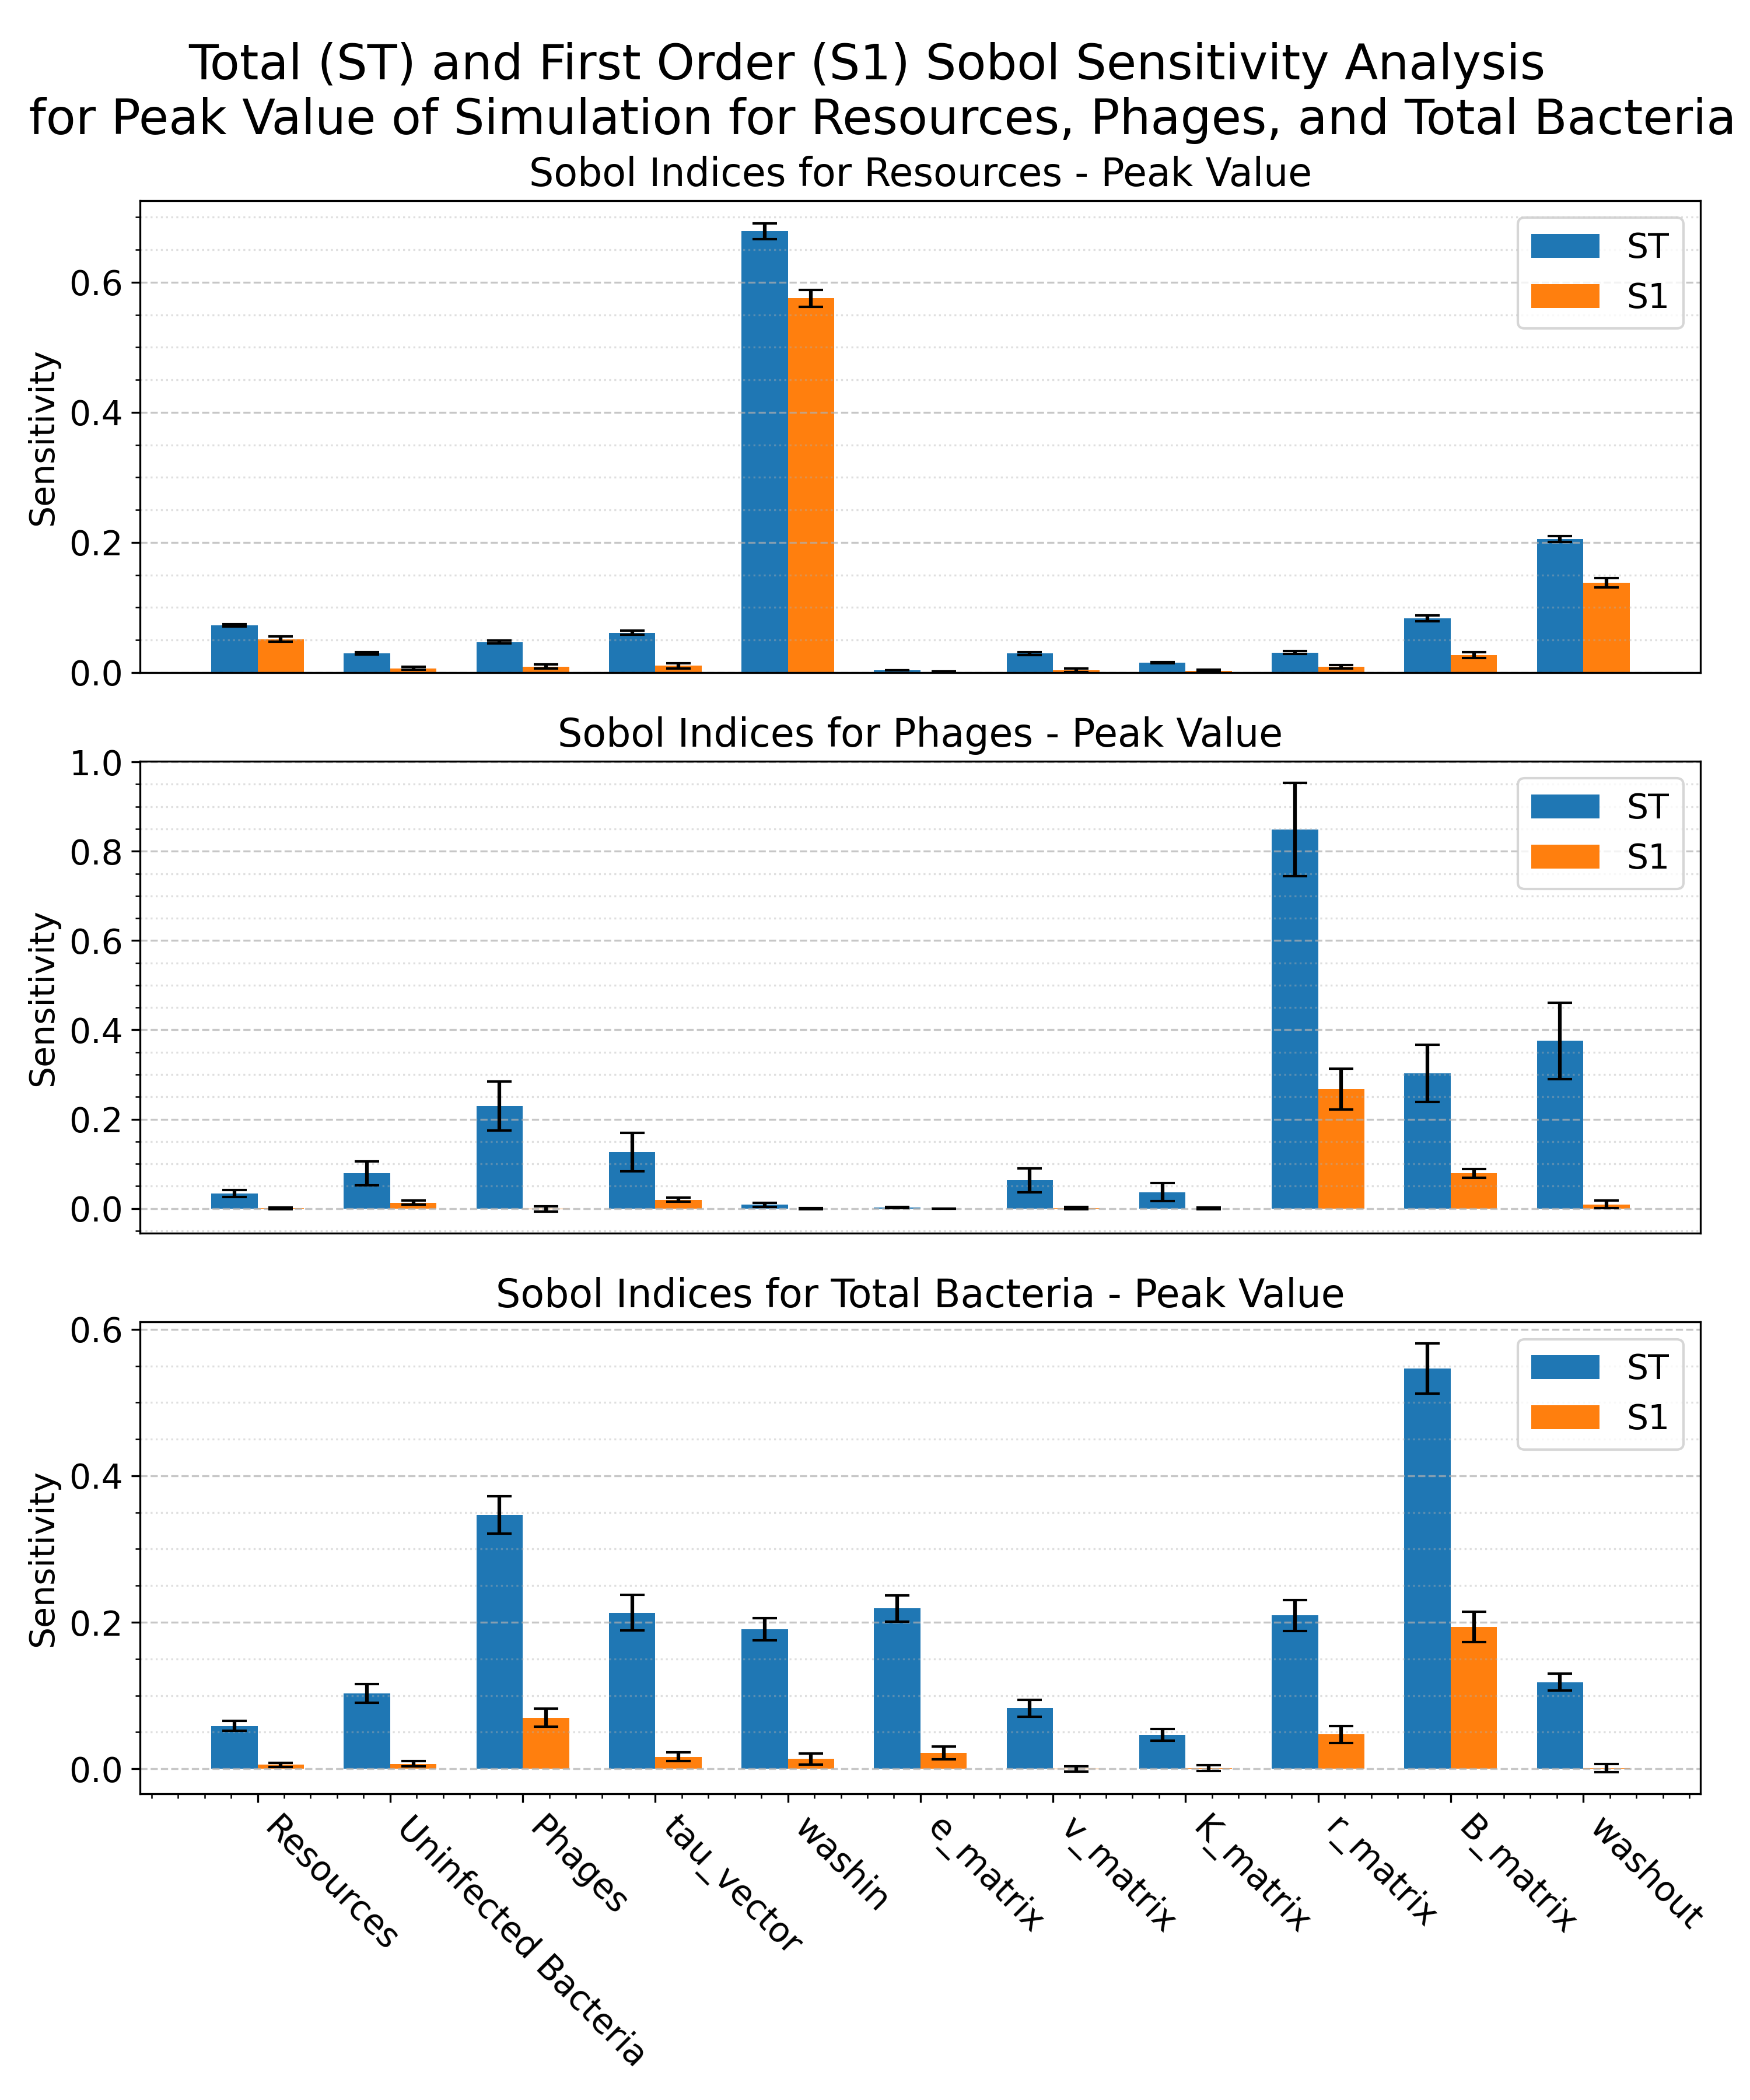
\includegraphics[width=\linewidth]{Plots/Created/SOBOL/SOBOL_analysis_1749149674_Peak.png}
        \caption{
            Peak population value. 
        }
        \label{fig:created:Sobol_peak}
    \end{subfigure}
    \hfill
    \begin{subfigure}{0.32\linewidth}
        \centering
        \captionsetup{width=1\linewidth}
        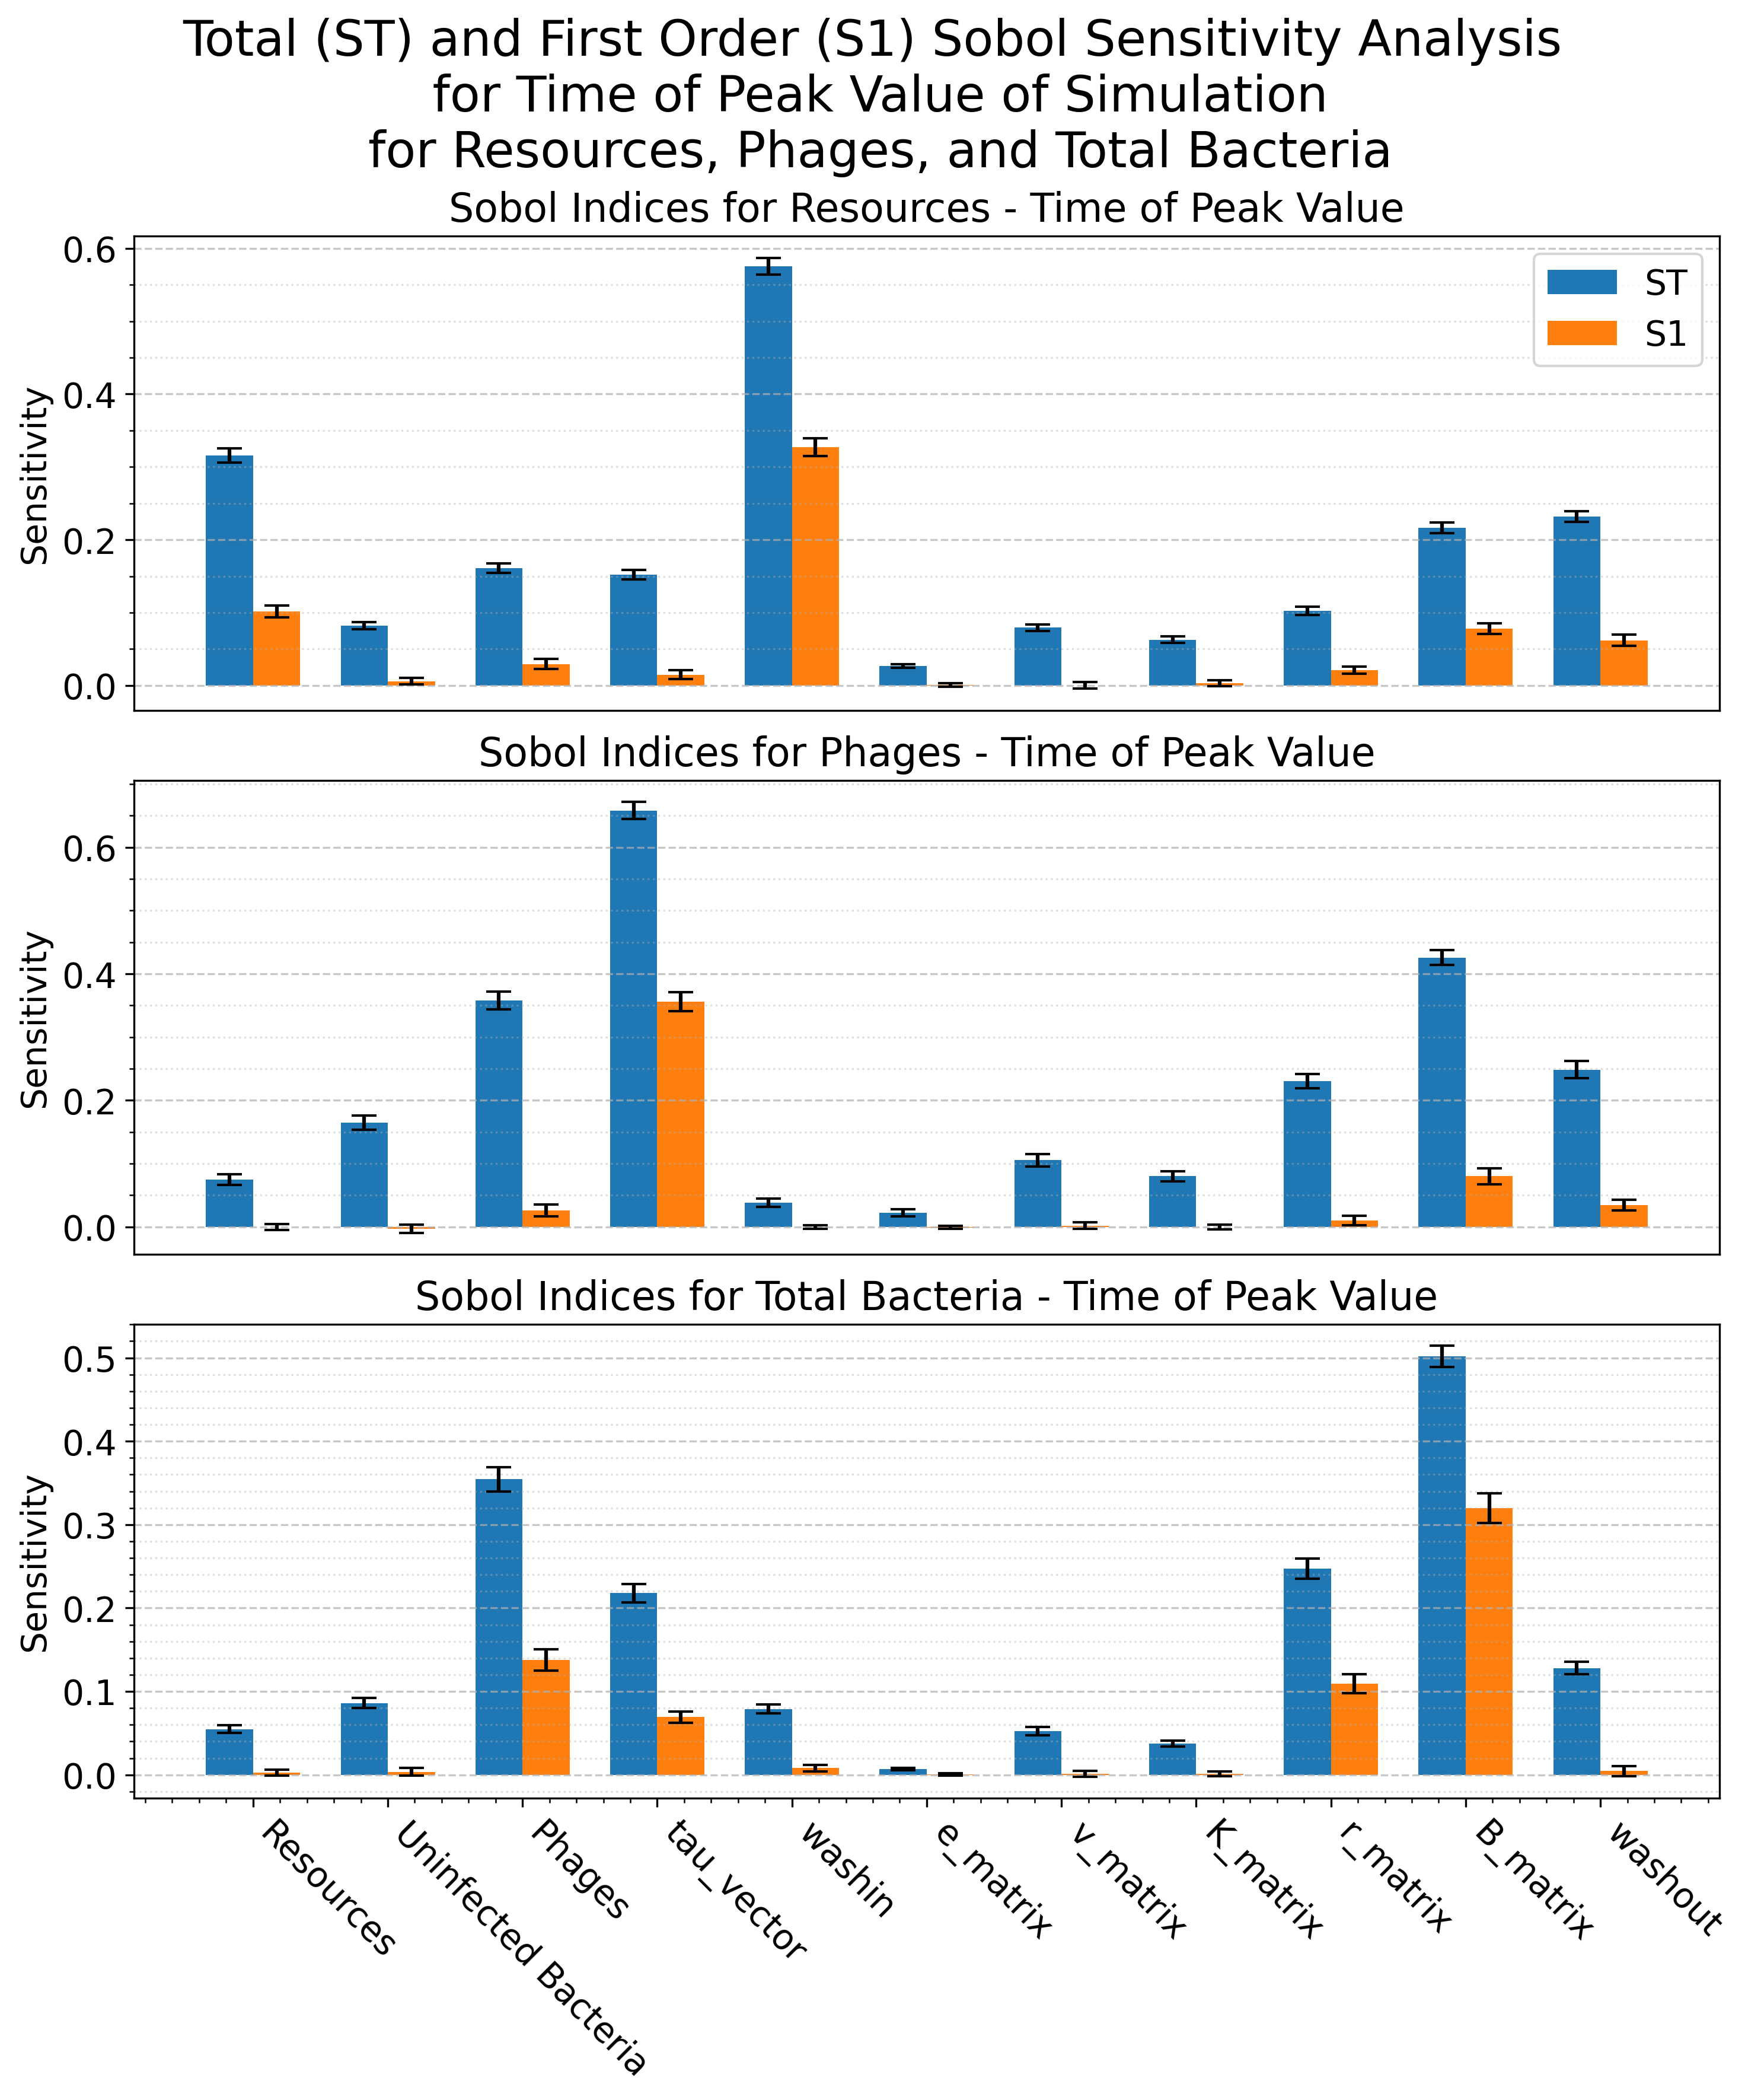
\includegraphics[width=\linewidth]{Plots/Created/SOBOL/SOBOL_analysis_1749149674_Time_of_Peak.png}
        \caption{
            Time at peak population. 
        }
        \label{fig:created:Sobol_peak_time}
    \end{subfigure}
    \caption{
            Sobol analyses for the final, peak, and time of peak value with a washin and washout rate. 
            The data was saved from the dashboard and plotted using Matplotlib. 
            The values used for this Sobol test can be found in \Cref{tab:appendixE:Sobol_analysis_values}. 
        }
    \label{fig:created:Sobol_analyses}
\end{figure}

\section{Why 95\%?}
\label{sec:appendixF:why_95}
The 95\% rule helps in the IVA analysis. 
Due to the solver, when taking the absolute peak value, the same time value can occur multiple times. 
Alternatively, in an ever-increasing value, such as phages, the peak values occur at the last time step of the simulation, or they plateau and no longer grow. 
However, as the parameter value changes, each graph for every input change will change the growth rate of the entity, changing how fast the entity population grows. 

\Cref{fig:appendixF:IVA_95_vs_100} shows how using the 95\% rule vs the 100\% rule for finding the max value reached helps smooth out computational errors from the ODE solver and smooths out the shape. 
For the phages, using the 100\% rule (\Cref{fig:appendixF:IVA_phages_100}) shows that the population peaked at the end of the simulation, $t=15$, for all $e$ values. 
However, at $t=15$, the population plateaued, as evident by the line graph. 
Plotting the same plot but calculating the peak at 95\% of the actual peak (\Cref{fig:appendixF:IVA_phage_95}) shows that the green line ($e=0.25$) “reached” its peak at $t=8.4$ before the red line ($e=0.05$) at $t=9.4$, a whole unit of time after $e=0.25$. 
The user can thus conclude that, for this instance, larger $e$ values will cause the phage population to reach its “peak” faster than smaller $e$ values. 

\Cref{fig:appendixF:IVA_uninfected_bacteria_95} and \Cref{fig:appendixF:IVA_uninfected_bacteria_100} likewise show how the 95\% rule can improve analysis of the change in time of peak. 
\Cref{fig:appendixF:IVA_uninfected_bacteria_100} shows how the peak is reached at set time values. 
Due to how \textit{solve\_ivp()} from SciPy works, it automatically chooses time values that it thinks would best capture the dynamics of the system without calculating too many steps. 
The user can control the step size by adjusting the absolute and relative error bounds, as well as by minimizing the time step size. 
The user can also specify their time range, along with the number of steps to run, thereby increasing control over the chosen time values. 
It takes approximately 0.02321 seconds to simulate 15-time units, where 200-time steps are selected and solved by the solver. 
Comparatively, a simulation with 1000 time units and 1000000 (a 5000x increase in samples) equidistant time samples takes about 1.71651 seconds to run, a 73.95562258x increase in time spent computing the simulation. 
The total time taken to run the entire method call, including a call to the simple graph maker at the top of the dashboard, was 1.76130 seconds, compared to 17.70634 seconds. 

Alternatively, instead of controlling the solver, the user can use the 95\% rule.
Although some accuracy is lost. 
Going from the 100\% rule to the 95\% rule, the solver still captures the peak values and the dynamics, but the accuracy is lost. 
The 100\% rule shows that for $e=0.25$, the time the uninfected population reached its peak occurred at $t=3.2$. 
However, for the 95\% rule, the time at which the peak occurred at $t=3.05$. 
The slope (the $a$ value) and the intercept (the $c$ value) are somewhat similar, with very high and similar $R^2$ values (0.97), suggesting a good linear fit of the data. 

\Cref{fig:appendixF:IVA_uninfected_bacteria_100_own_time} illustrates how increasing the time sampling to a more fine-grained level yields a more accurate graph. 
Instead of having the solver choose the time values to test, 1000 equidistant time values were selected between 0 and 15. 
The solver can more accurately calculate the population values and calculate the proper time of peak. 
Comparing the 100\% rule without the custom time values with the 100\% rule with the custom time values shows that the same time values were calculated. 
In both, $e=0.25$ resulted in a time of peak at 3.2, and for $e=0.05$, the time of peak occurred at $t=3.95$. 
This is in stark contrast to the 95\% rule vs 100\% rule without the custom time, showing a difference of $0.15$ time units. 
The custom time values also preserved the shape of the curve $e$-value vs. time curve, being almost identical to that of the 95\% rule as seen in \Cref{fig:appendixF:IVA_uninfected_bacteria_95} and \Cref{fig:appendixF:IVA_uninfected_bacteria_100_own_time}. 

Another issue that arises with the custom time is that it does not solve the issue seen with the phages, where the time of peak is at $t=15$. 

The user can control the \% rule with a value input on the dashboard. 
They can select to use the 95\% rule, 100\% rule, or even 83\% rule if they want by changing the value they use. 
The user can use their own custom time values to ensure that they get high-quality curves. 

\begin{figure}
    \centering
    \begin{subfigure}{1\linewidth}
        \centering
        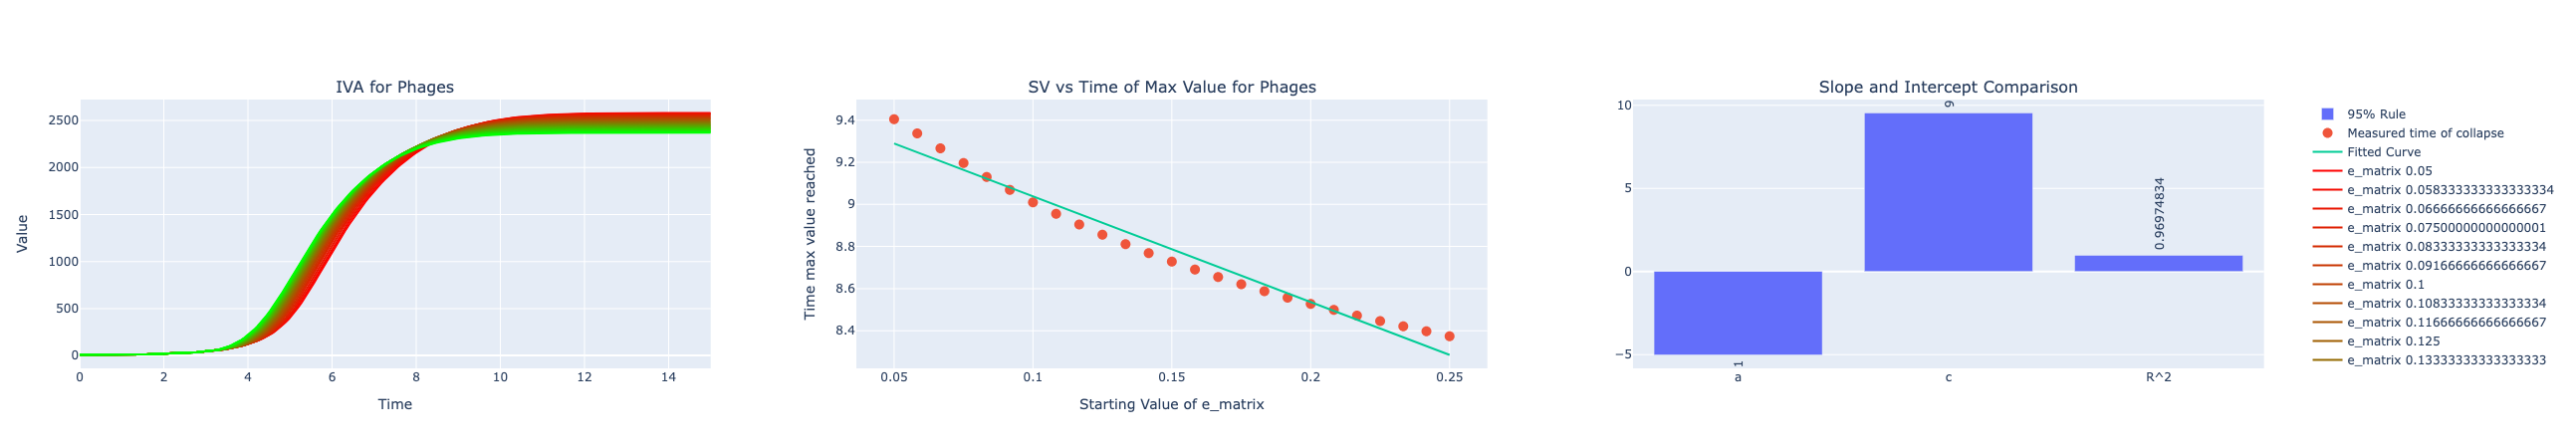
\includegraphics[width=\linewidth]{Plots/Created/IVA/initial_value_analysis_Phages_95.png}
        \caption{
            IVA for phage population, 95\% rule
        }
        \label{fig:appendixF:IVA_phage_95}
    \end{subfigure}
    \hfill
    \begin{subfigure}{1\linewidth}
        \centering
        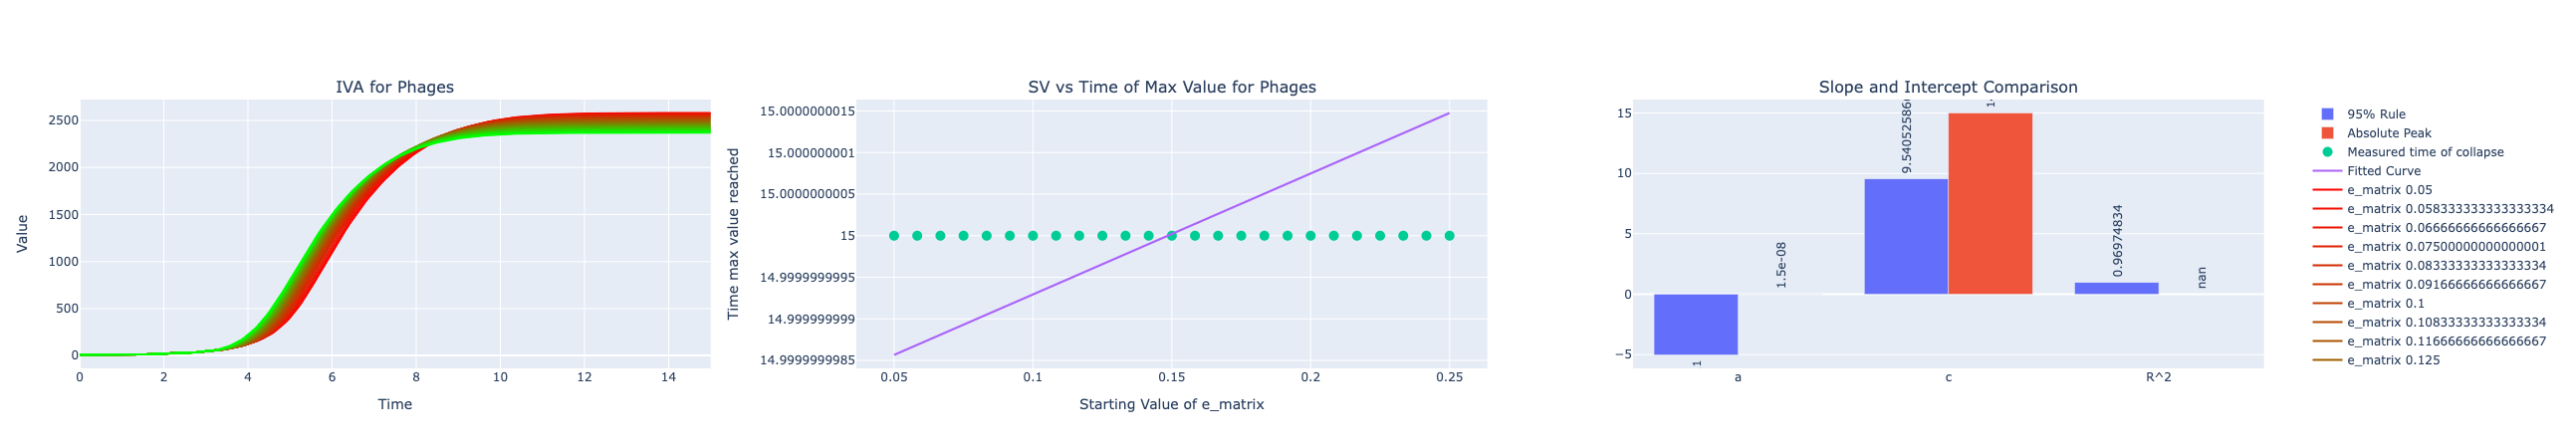
\includegraphics[width=\linewidth]{Plots/Created/IVA/initial_value_analysis_Phages_100.png}
        \caption{
            IVA for phage population, 100\% rule.  
        }
        \label{fig:appendixF:IVA_phages_100}
    \end{subfigure}
    \hfill
    \begin{subfigure}{1\linewidth}
        \centering
        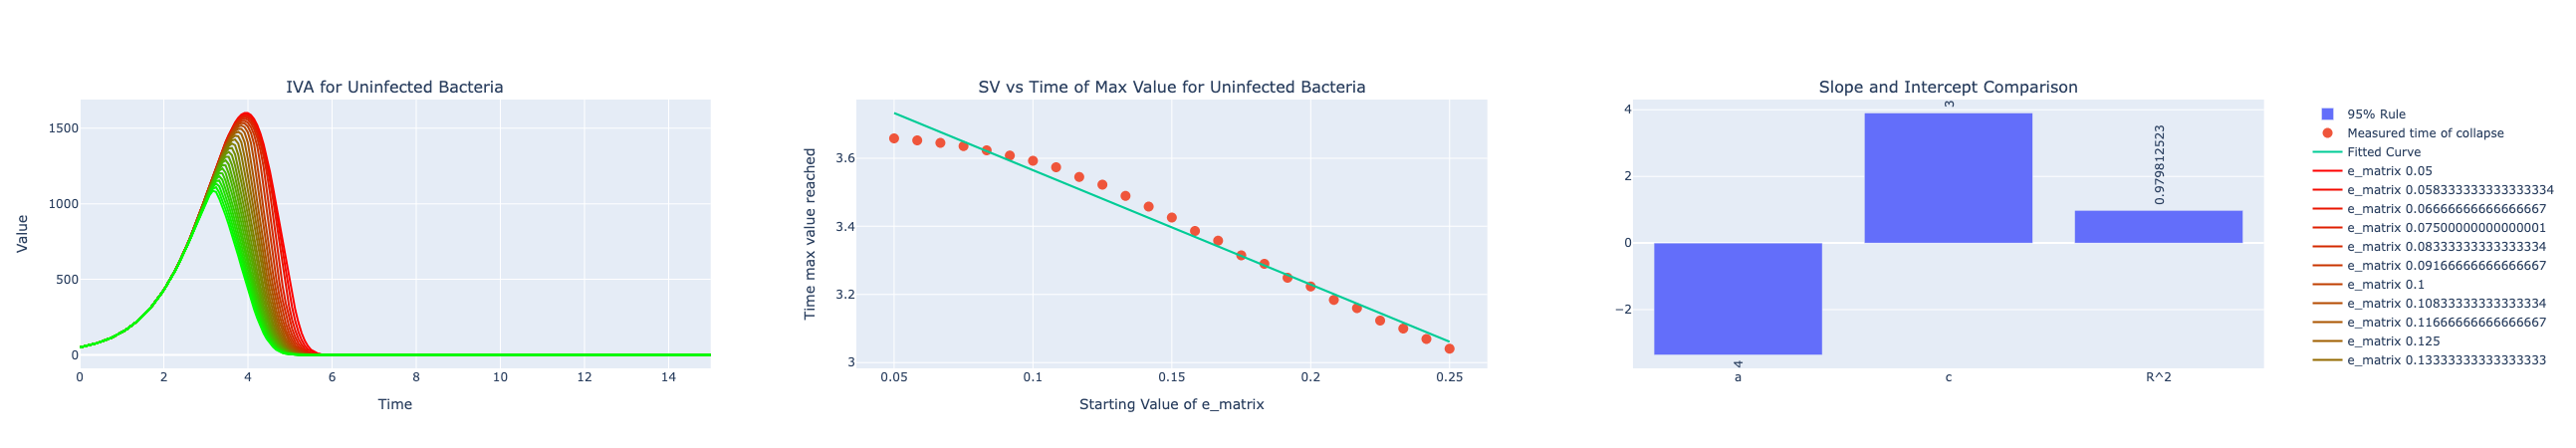
\includegraphics[width=\linewidth]{Plots/Created/IVA/initial_value_analysis_Uninfected_Bacteria_95.png}
        \caption{
            IVA for uninfected population, 95\% rule. 
        }
        \label{fig:appendixF:IVA_uninfected_bacteria_95}
    \end{subfigure}
    \hfill 
    \begin{subfigure}{1\linewidth}
        \centering
        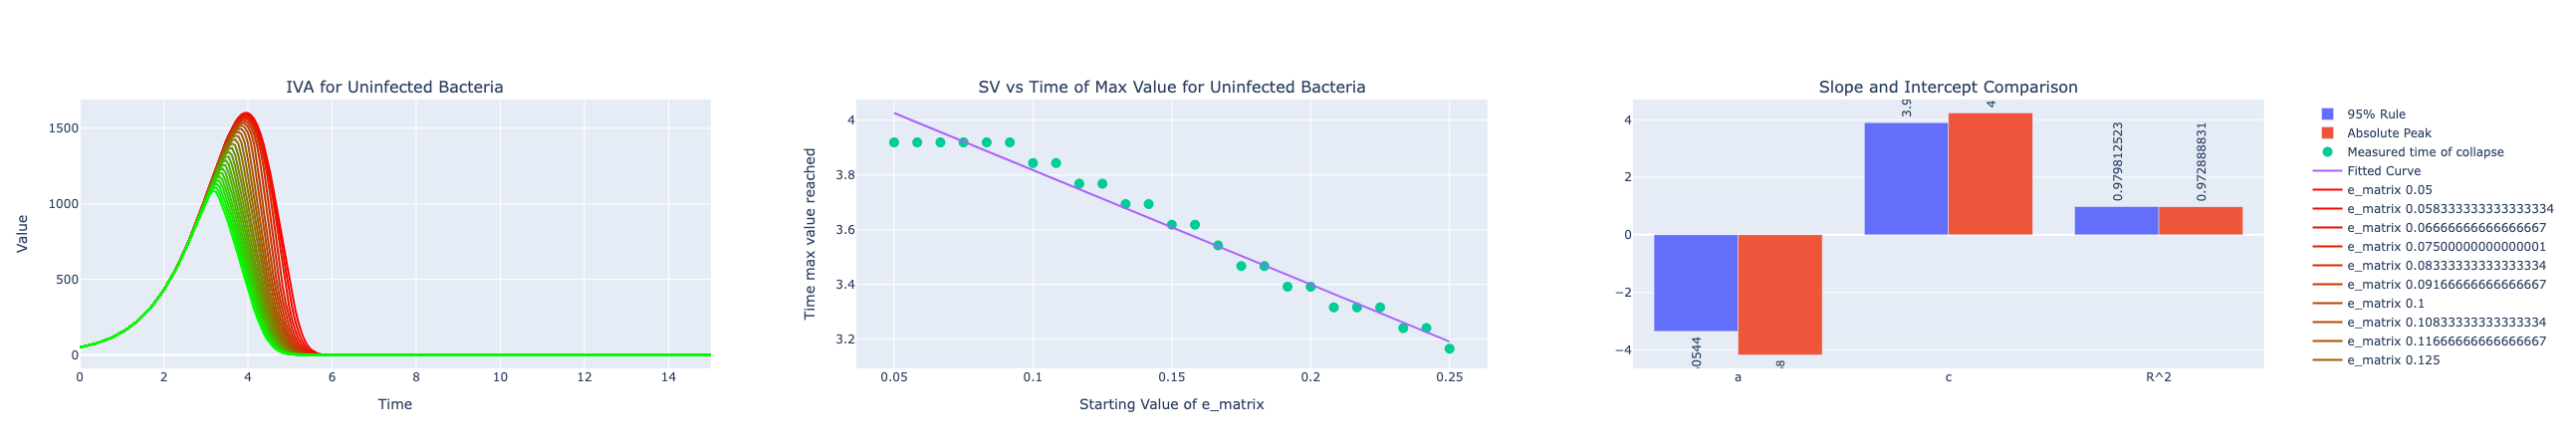
\includegraphics[width=\linewidth]{Plots/Created/IVA/initial_value_analysis_Uninfected_Bacteria_100.png}
        \caption{
            IVA for uninfected population, 100\% rule. 
        }
        \label{fig:appendixF:IVA_uninfected_bacteria_100}
    \end{subfigure}
    \begin{subfigure}{1\linewidth}
        \centering
        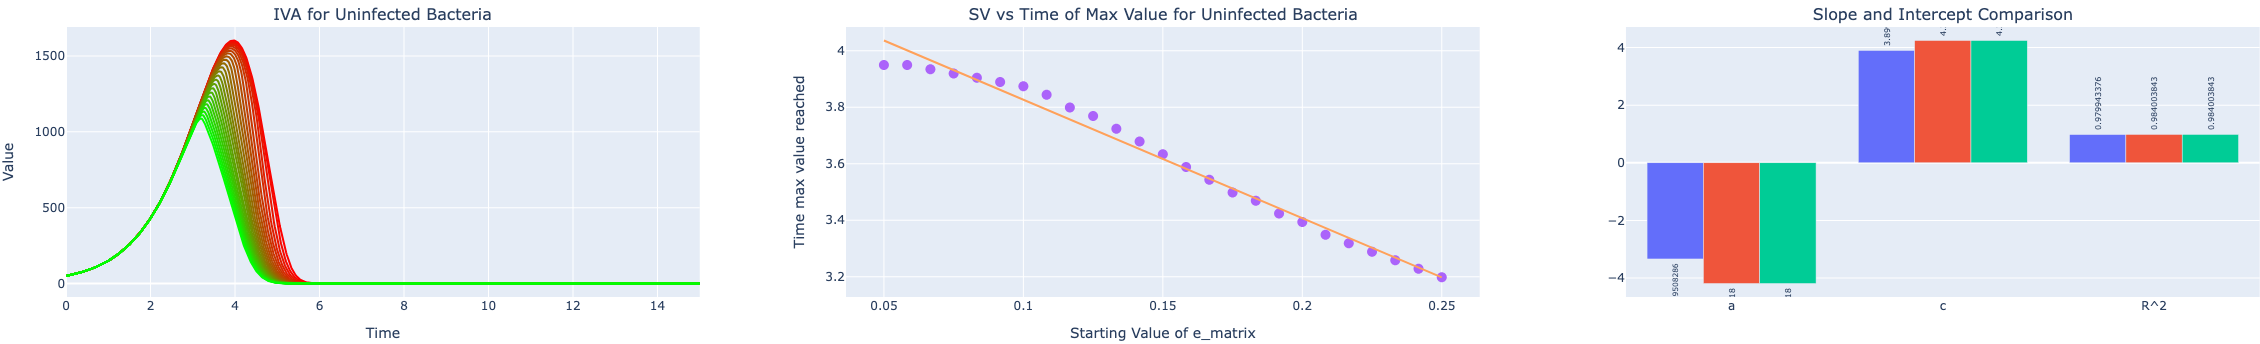
\includegraphics[width=\linewidth]{Plots/Created/IVA/initial_value_analysis_Uninfected_Bacteria_100_own_time.png}
        \caption{
            IVA for uninfected population, 100\% rule, 1000 equidistant time steps. 
        }
        \label{fig:appendixF:IVA_uninfected_bacteria_100_own_time}
    \end{subfigure}
    \caption{
        Testing the 95\% rule vs the 100\% rule, where the time at the absolute peak is taken and plotted in the second plot. 
        A comparison of phages and uninfected bacteria is shown. 
        Verification of the graph shape between the 95\% rule graph and a frequent time step with 100\% rule can be seen in c) and e). 
        The $e$ value is changed, ranging from 0.05 to 0.25. 
    }
    \label{fig:appendixF:IVA_95_vs_100}
\end{figure}

\section{Graph Behavior with IVA}
\label{sec:apendixF:graph_behavior_with_IVA}
\subsection{Resources $R$}
\begin{figure}[H]
    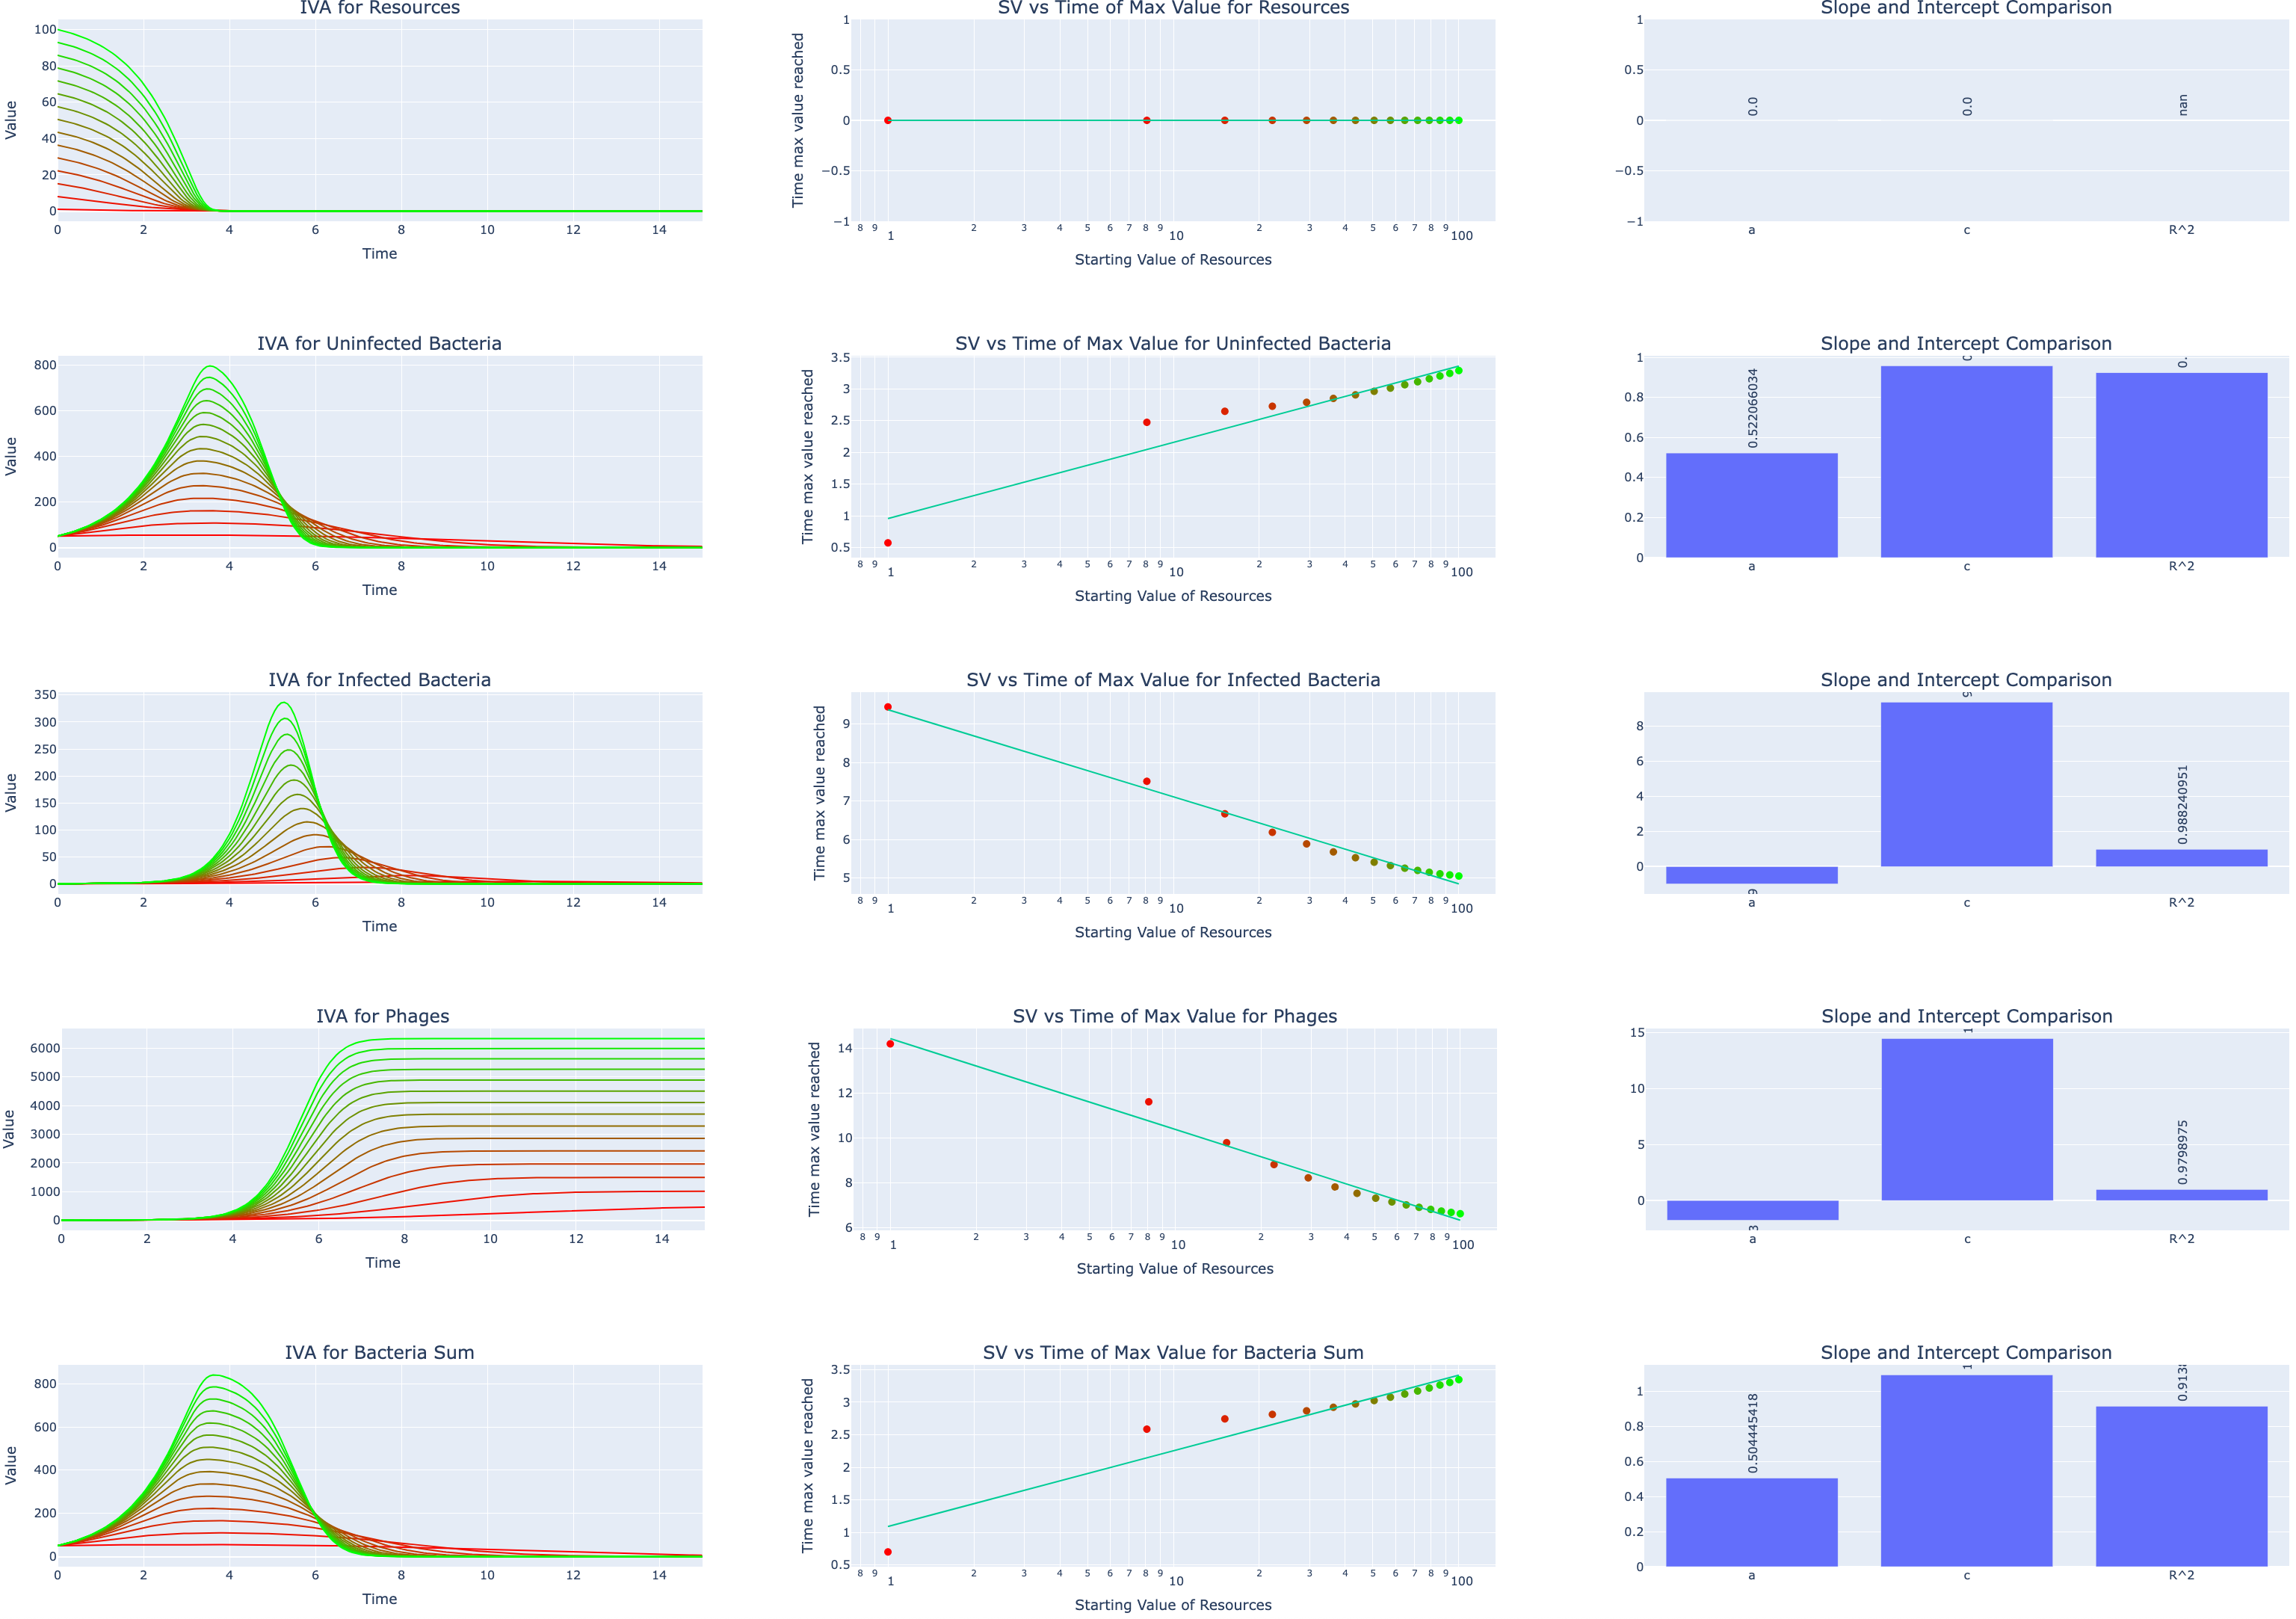
\includegraphics[width=1\textwidth]{Plots/Created/IVA/IVA_Table/resource_.png}
    \centering
    \caption{
        Changing initial resource values. 
    }
    \label{fig:created:IVA_IVAtable_resource}
\end{figure}

\subsection{Uninfected Bacteria $U$}
\begin{figure}[H]
    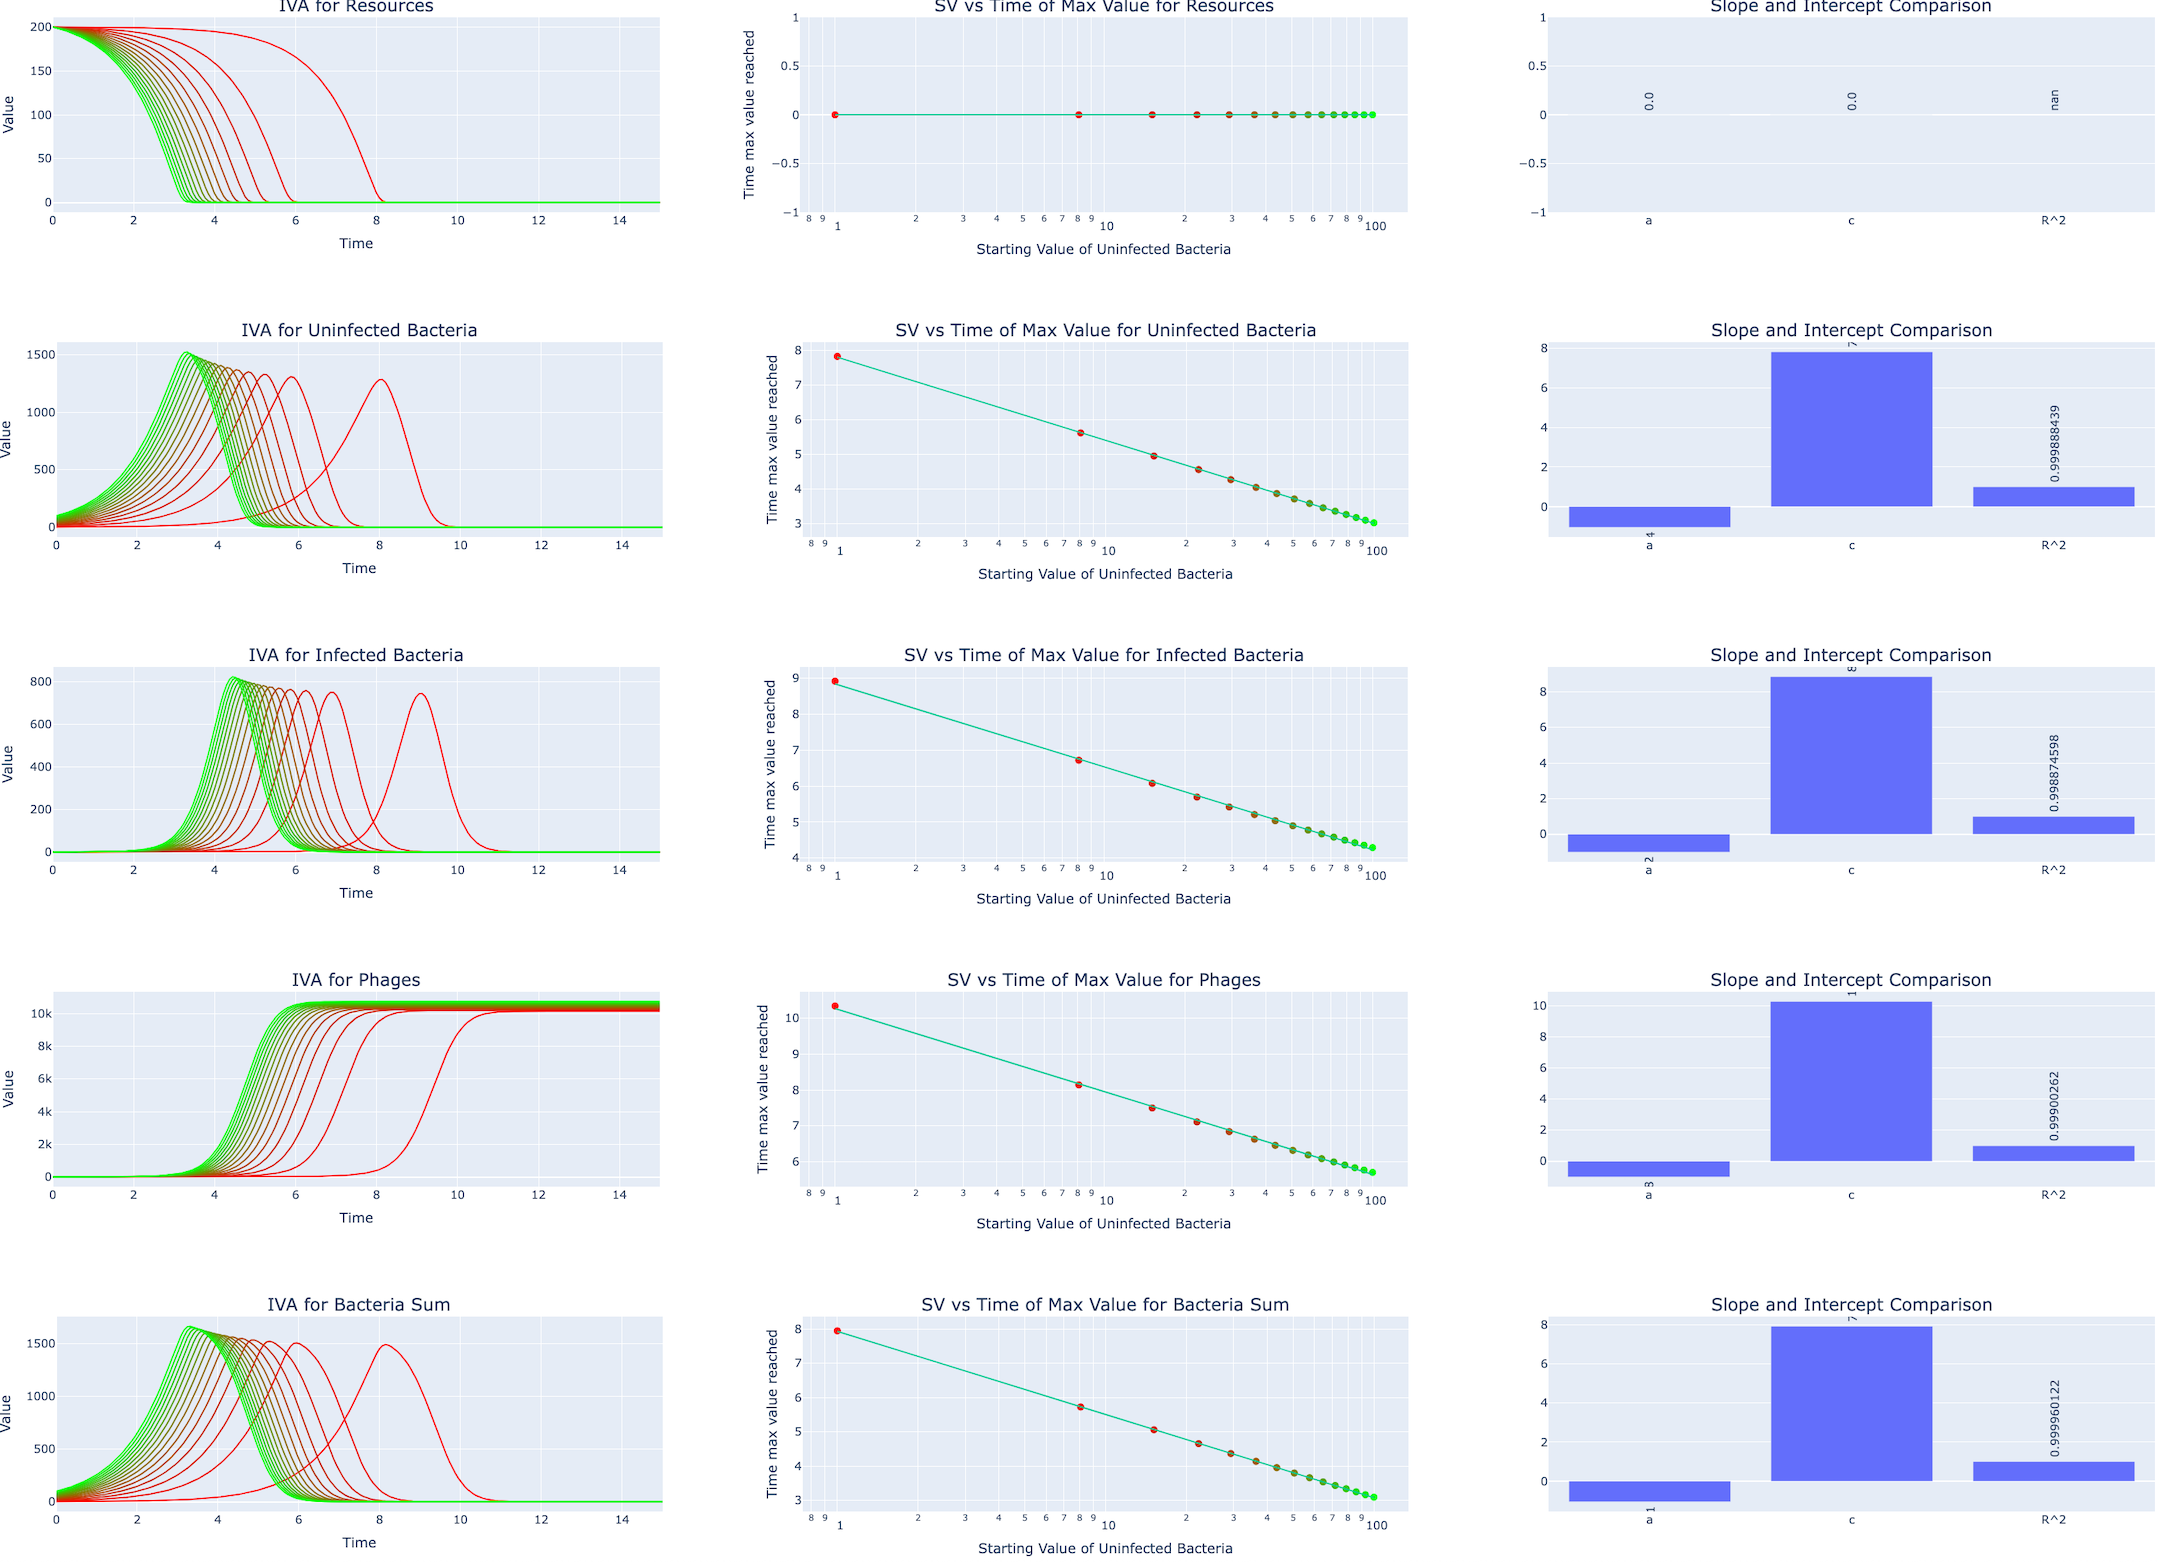
\includegraphics[width=1\textwidth]{Plots/Created/IVA/IVA_Table/uninfected_bacteria.png}
    \centering
    \caption{
        Changing initial uninfected bacteria values. 
    }
    \label{fig:created:IVA_IVAtable_uninfected_bacteria}
\end{figure}

\subsection{Phages $P$}
\begin{figure}[H]
    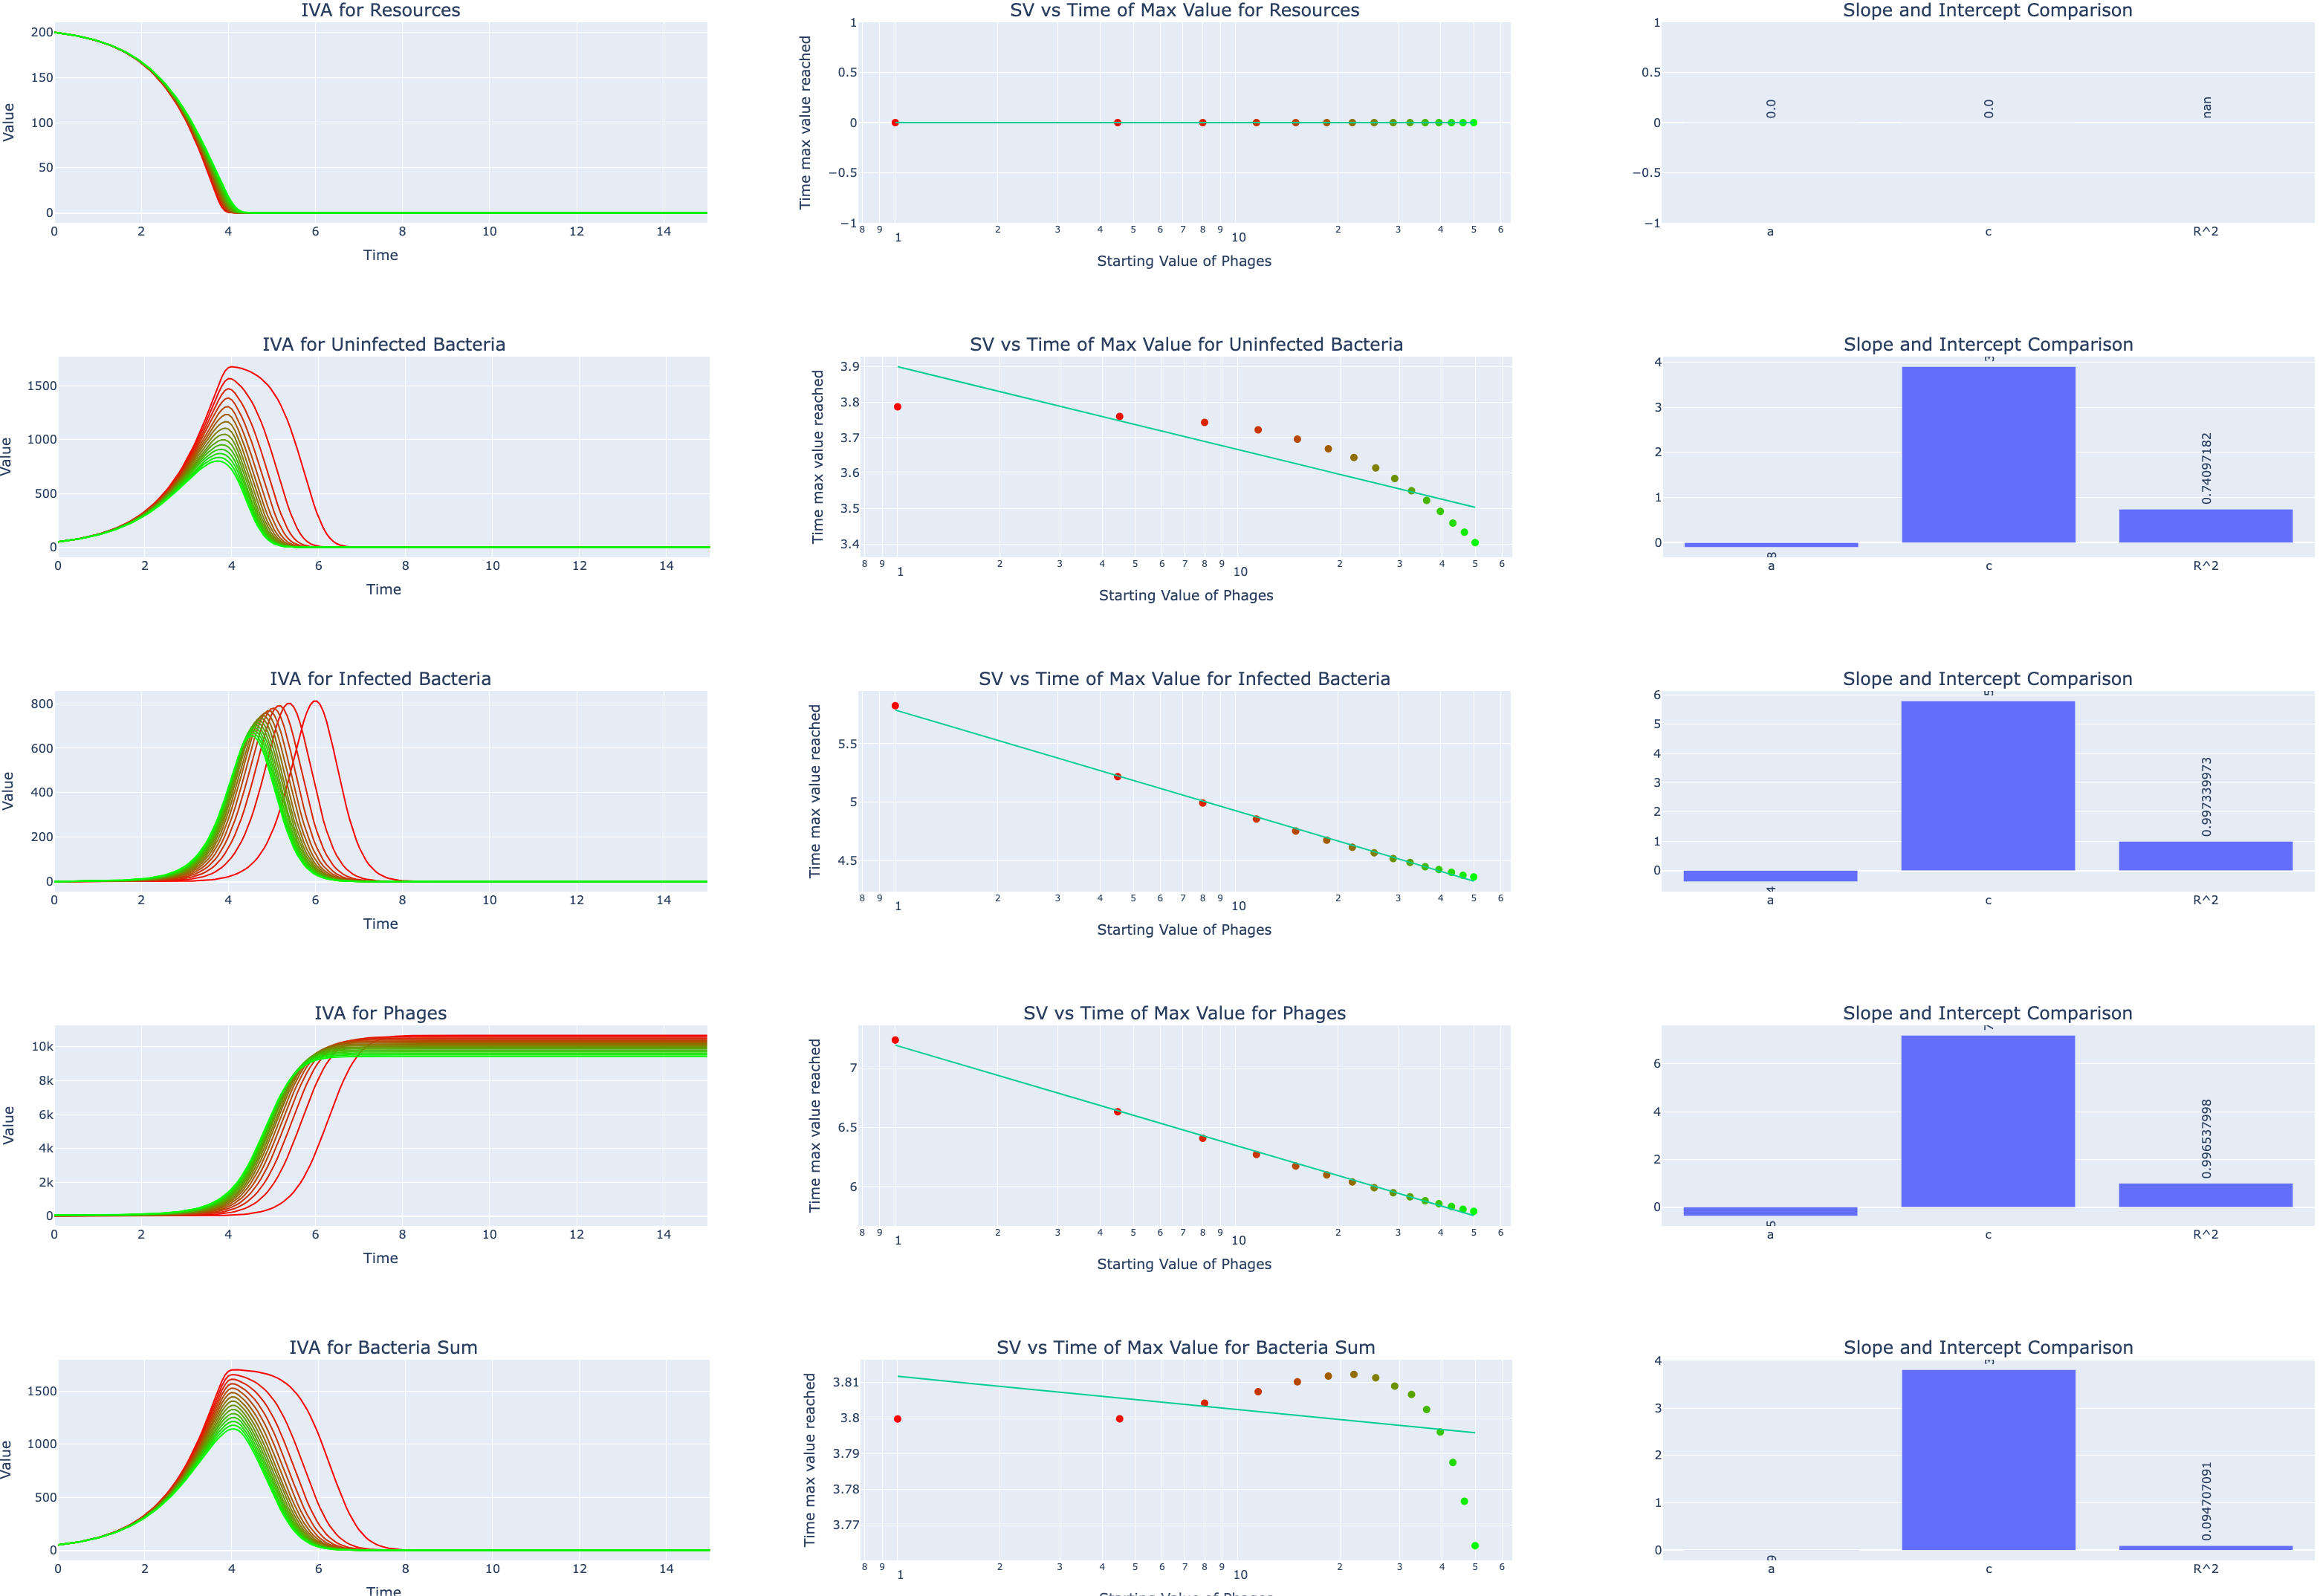
\includegraphics[width=1\textwidth]{Plots/Created/IVA/IVA_Table/phages.png}
    \centering
    \caption{
        Changing initial phage values. 
    }
    \label{fig:created:IVA_IVAtable_phages}
\end{figure}

\subsection{Latent Period $\tau$}
\begin{figure}[H]
    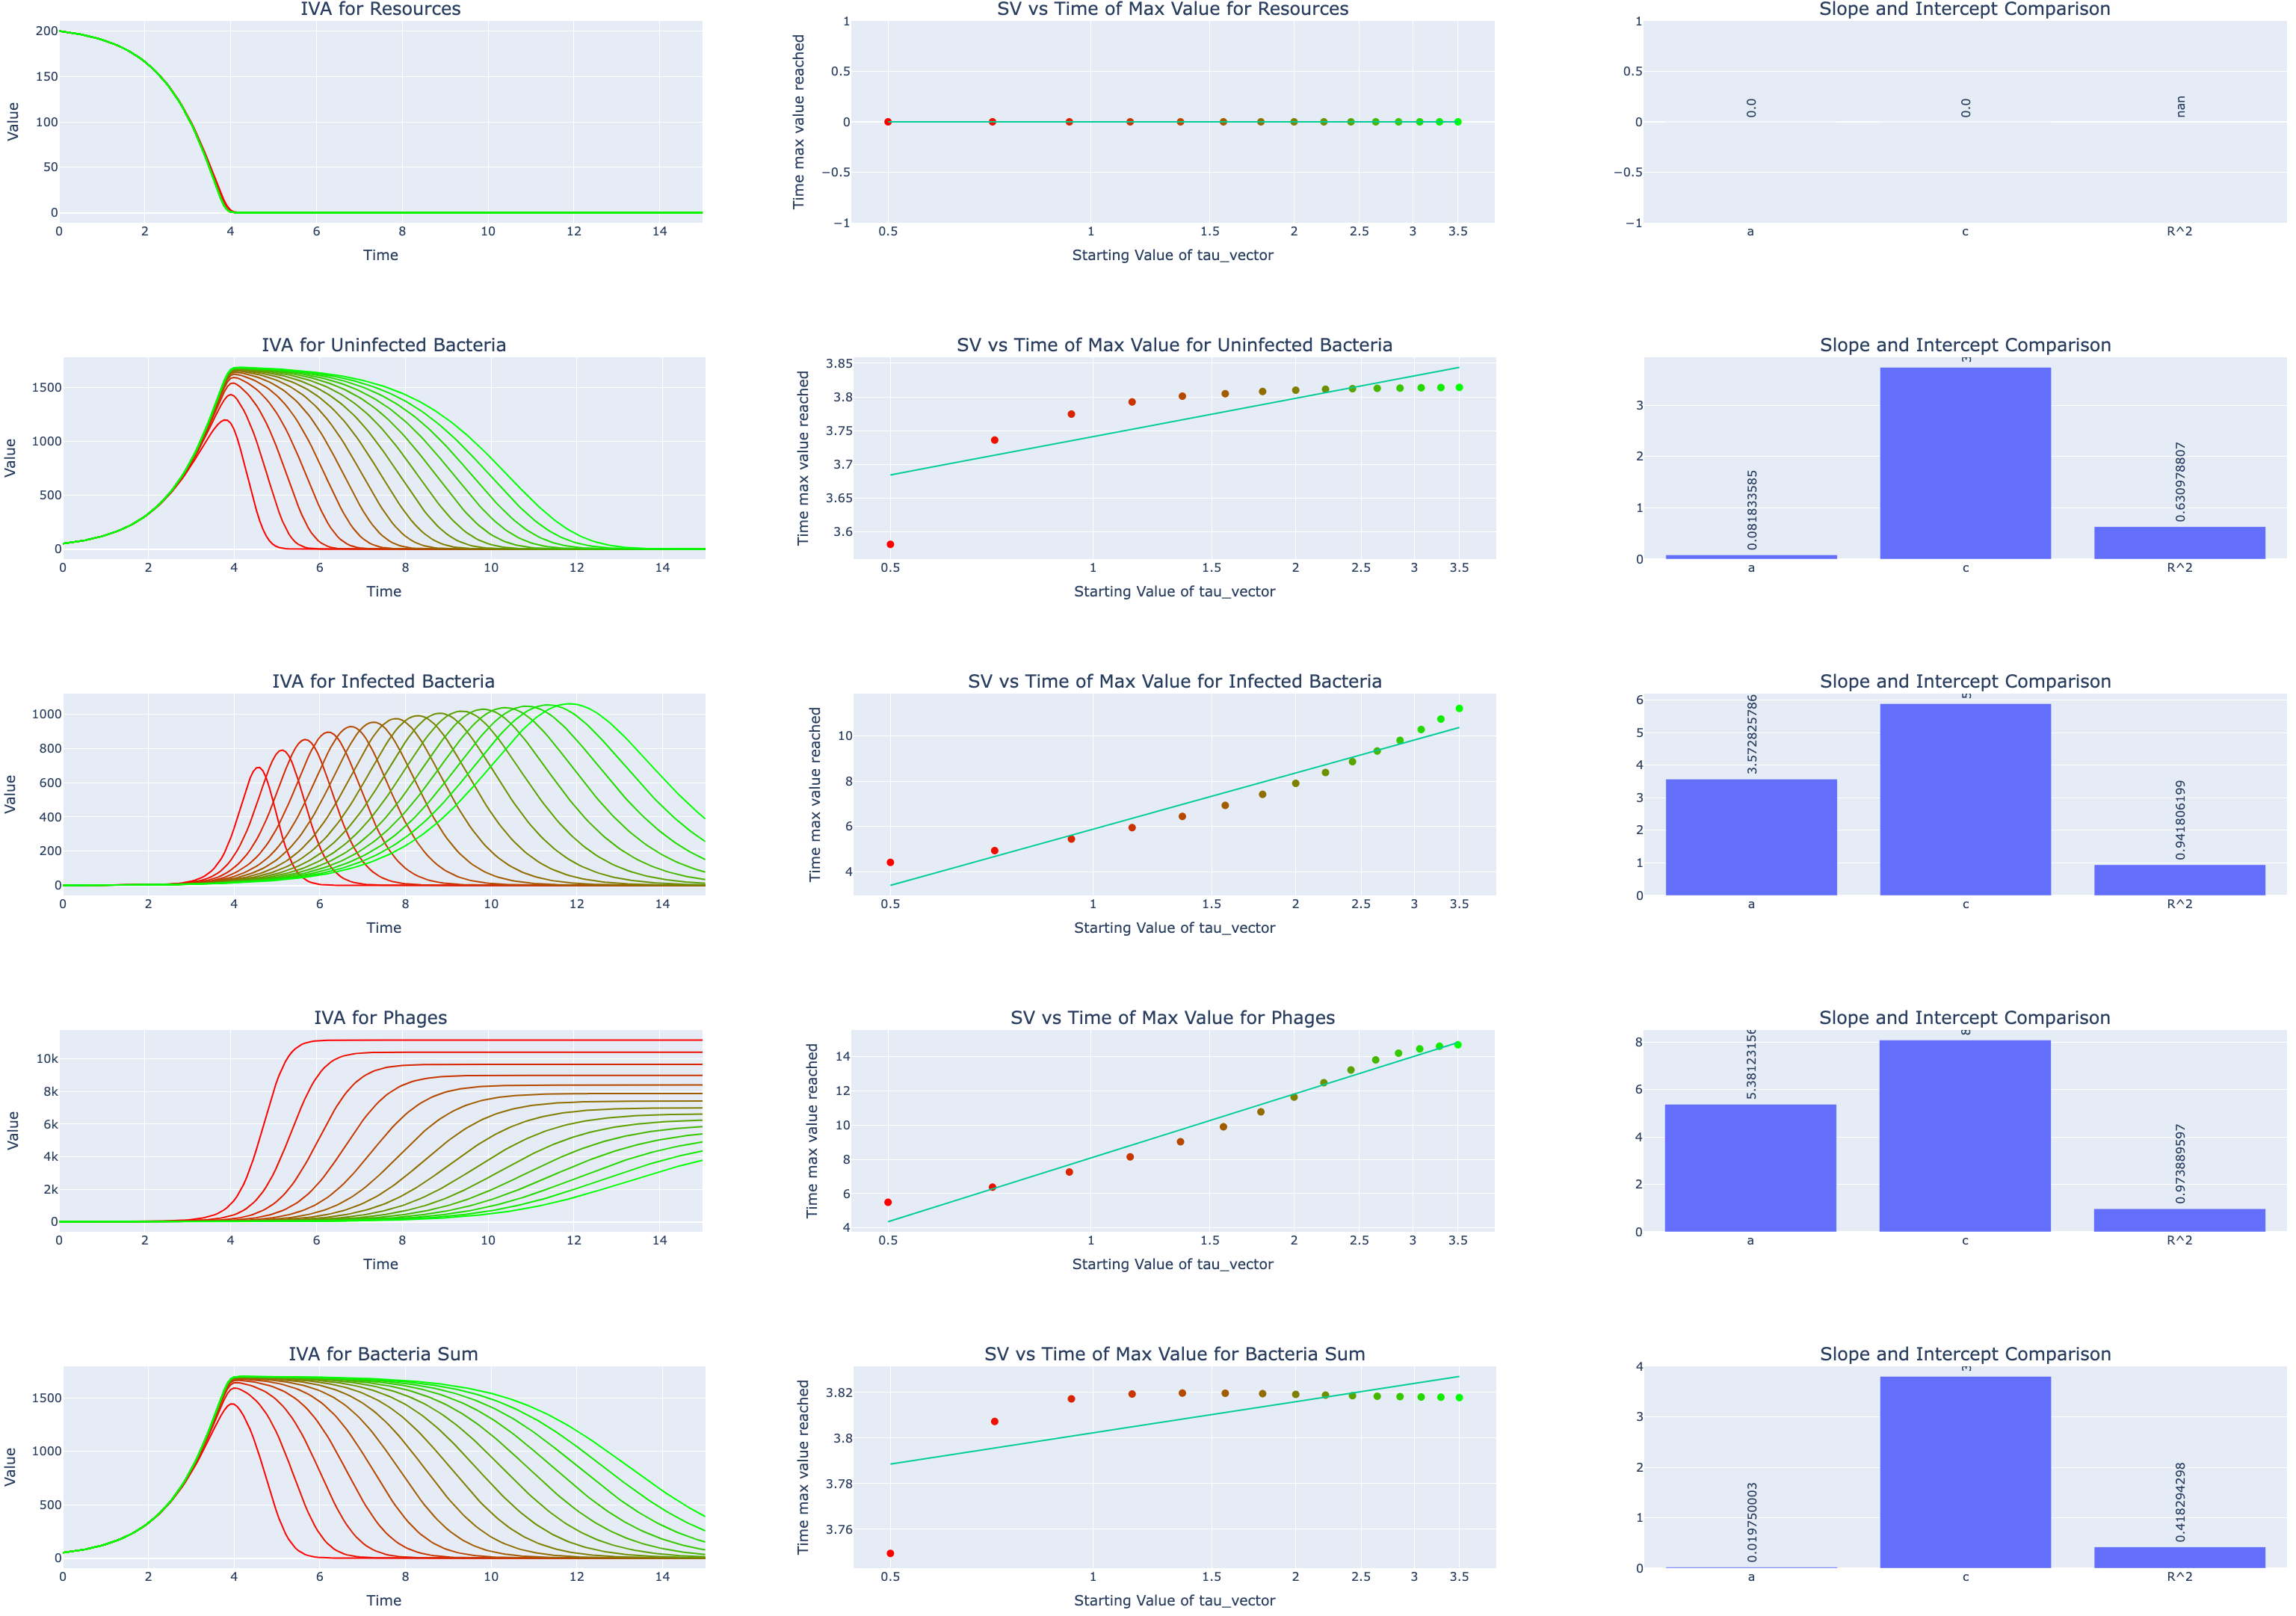
\includegraphics[width=1\textwidth]{Plots/Created/IVA/IVA_Table/tau.png}
    \centering
    \caption{
        Changing $\tau$ values. 
    }
    \label{fig:created:IVA_IVAtable_tau}
\end{figure}

\subsection{Phage Adsorption Rate $r$}
\begin{figure}[H]
    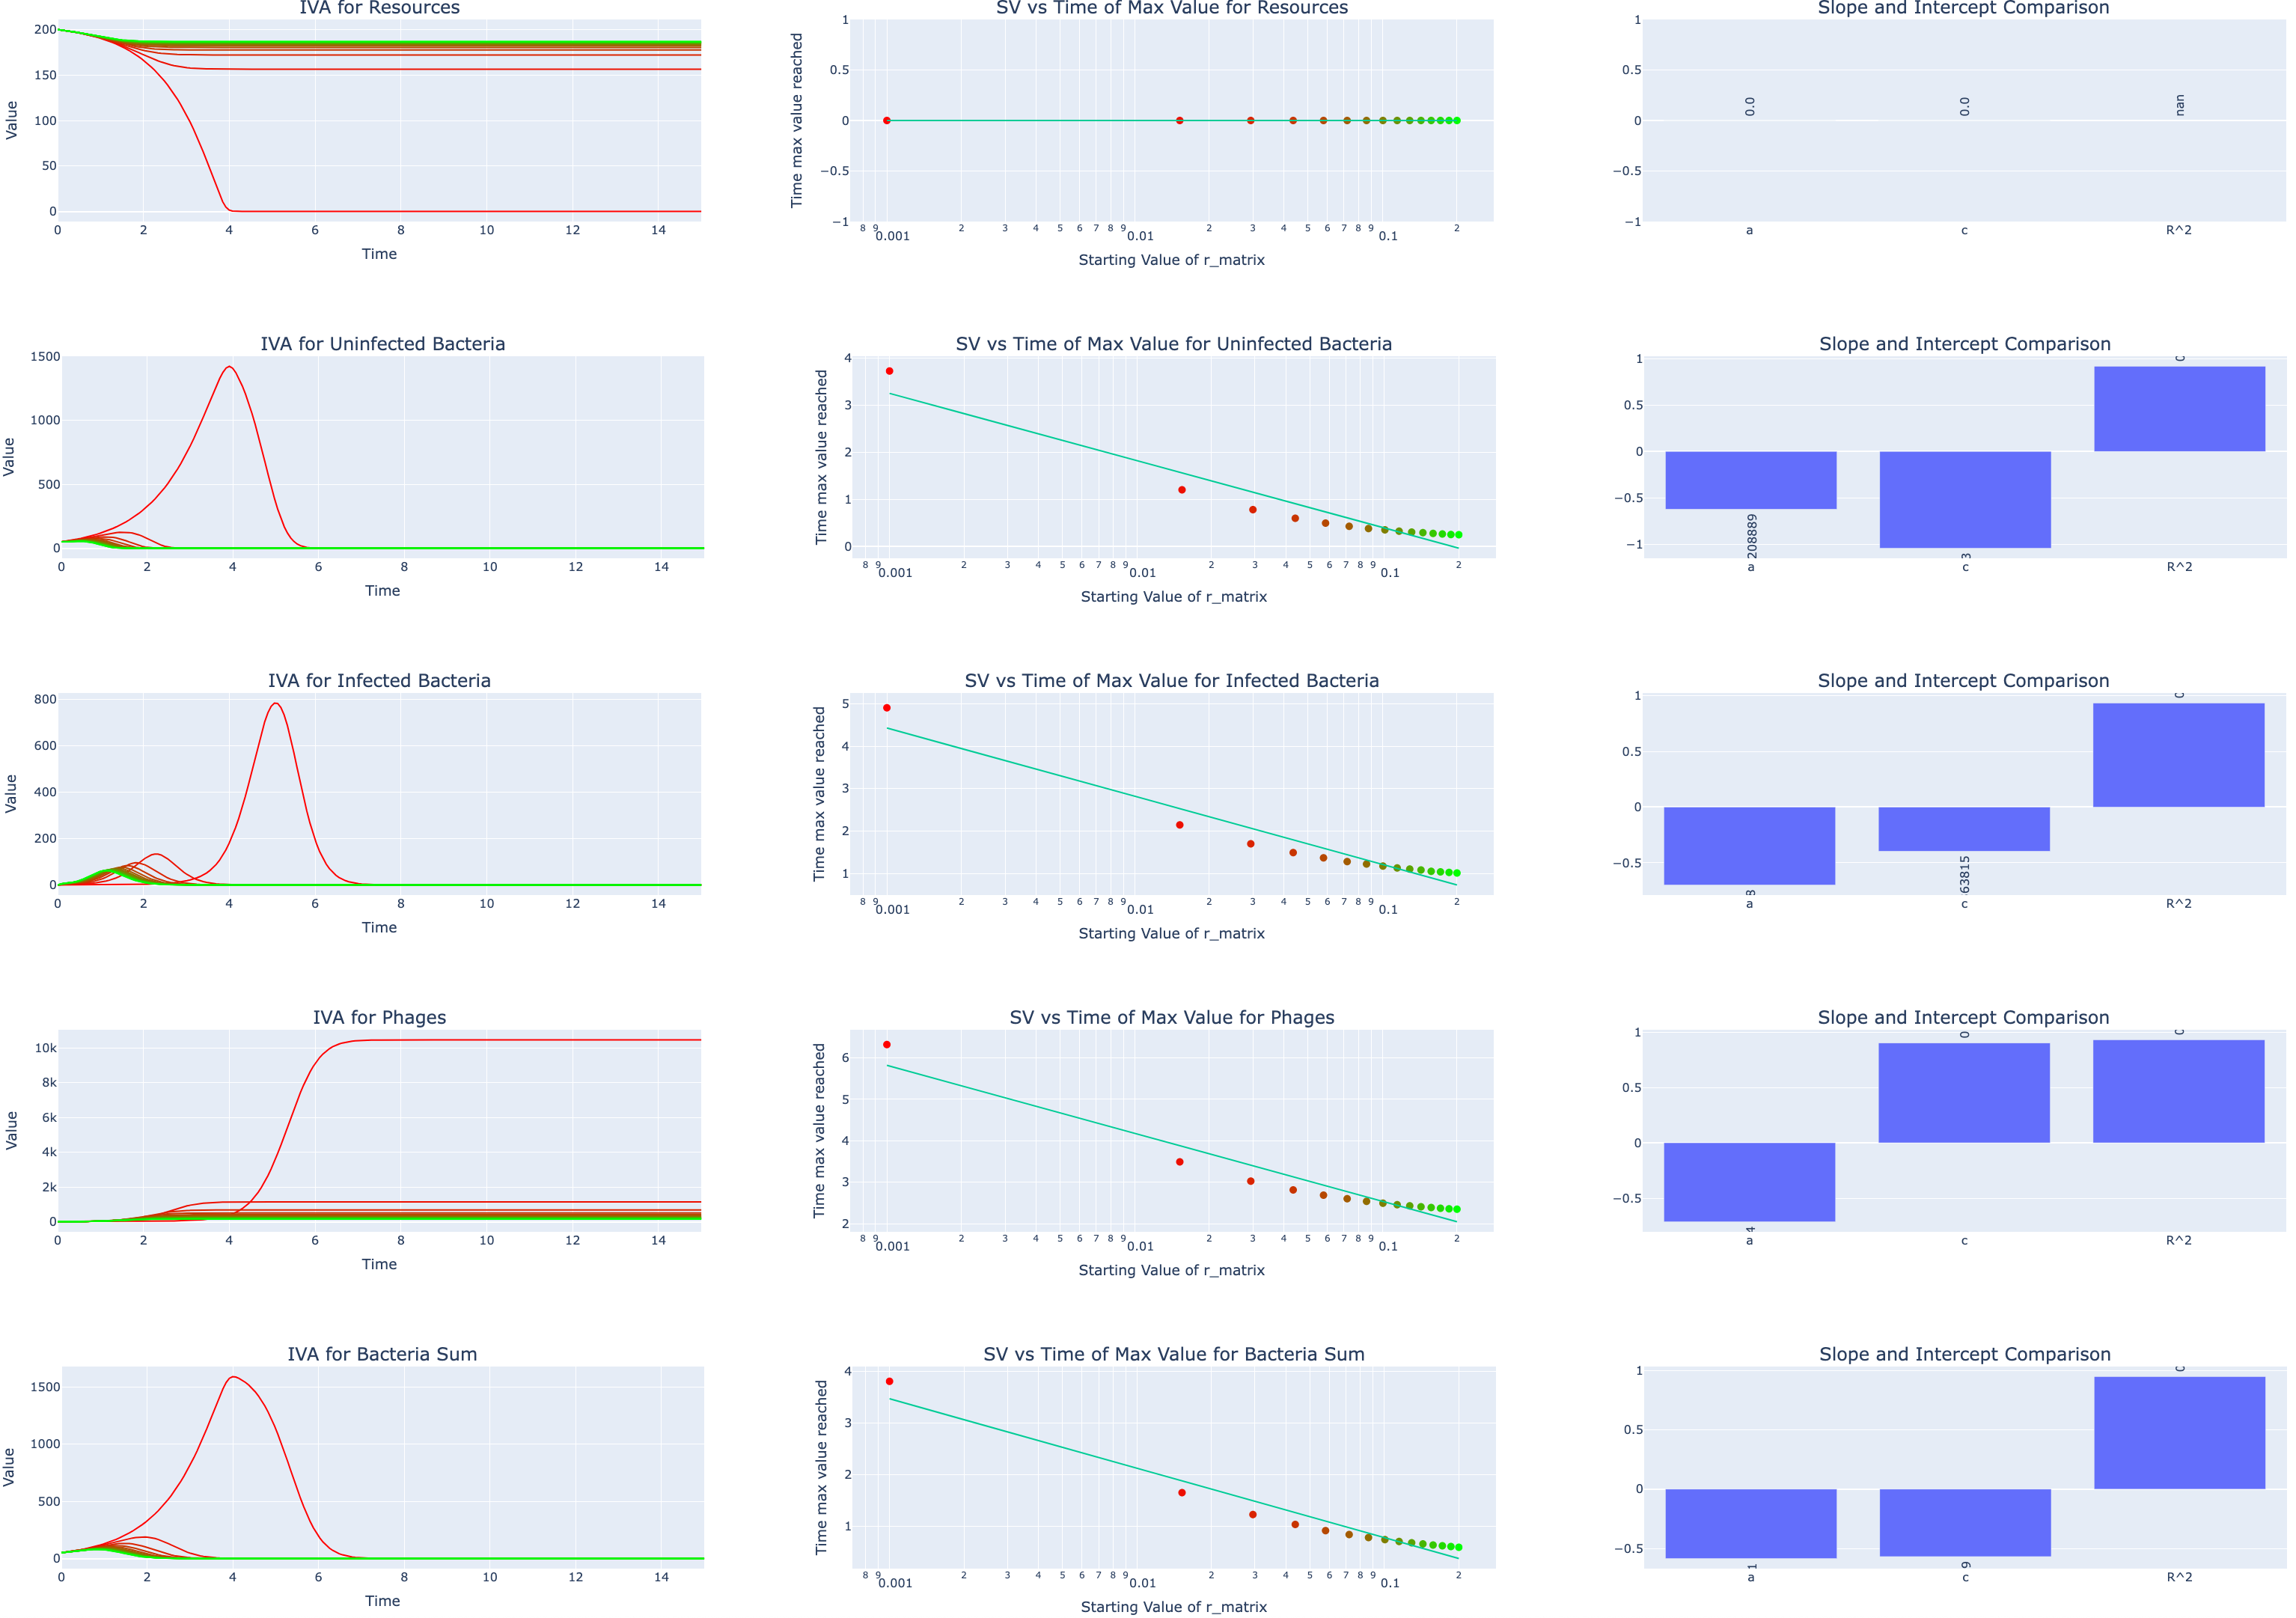
\includegraphics[width=1\textwidth]{Plots/Created/IVA/IVA_Table/r.png}
    \centering
    \caption{
        Changing initial $r$ values. 
    }
    \label{fig:created:IVA_IVAtable_r}
\end{figure}

\subsection{Burst Size $\beta$}
\begin{figure}[H]
    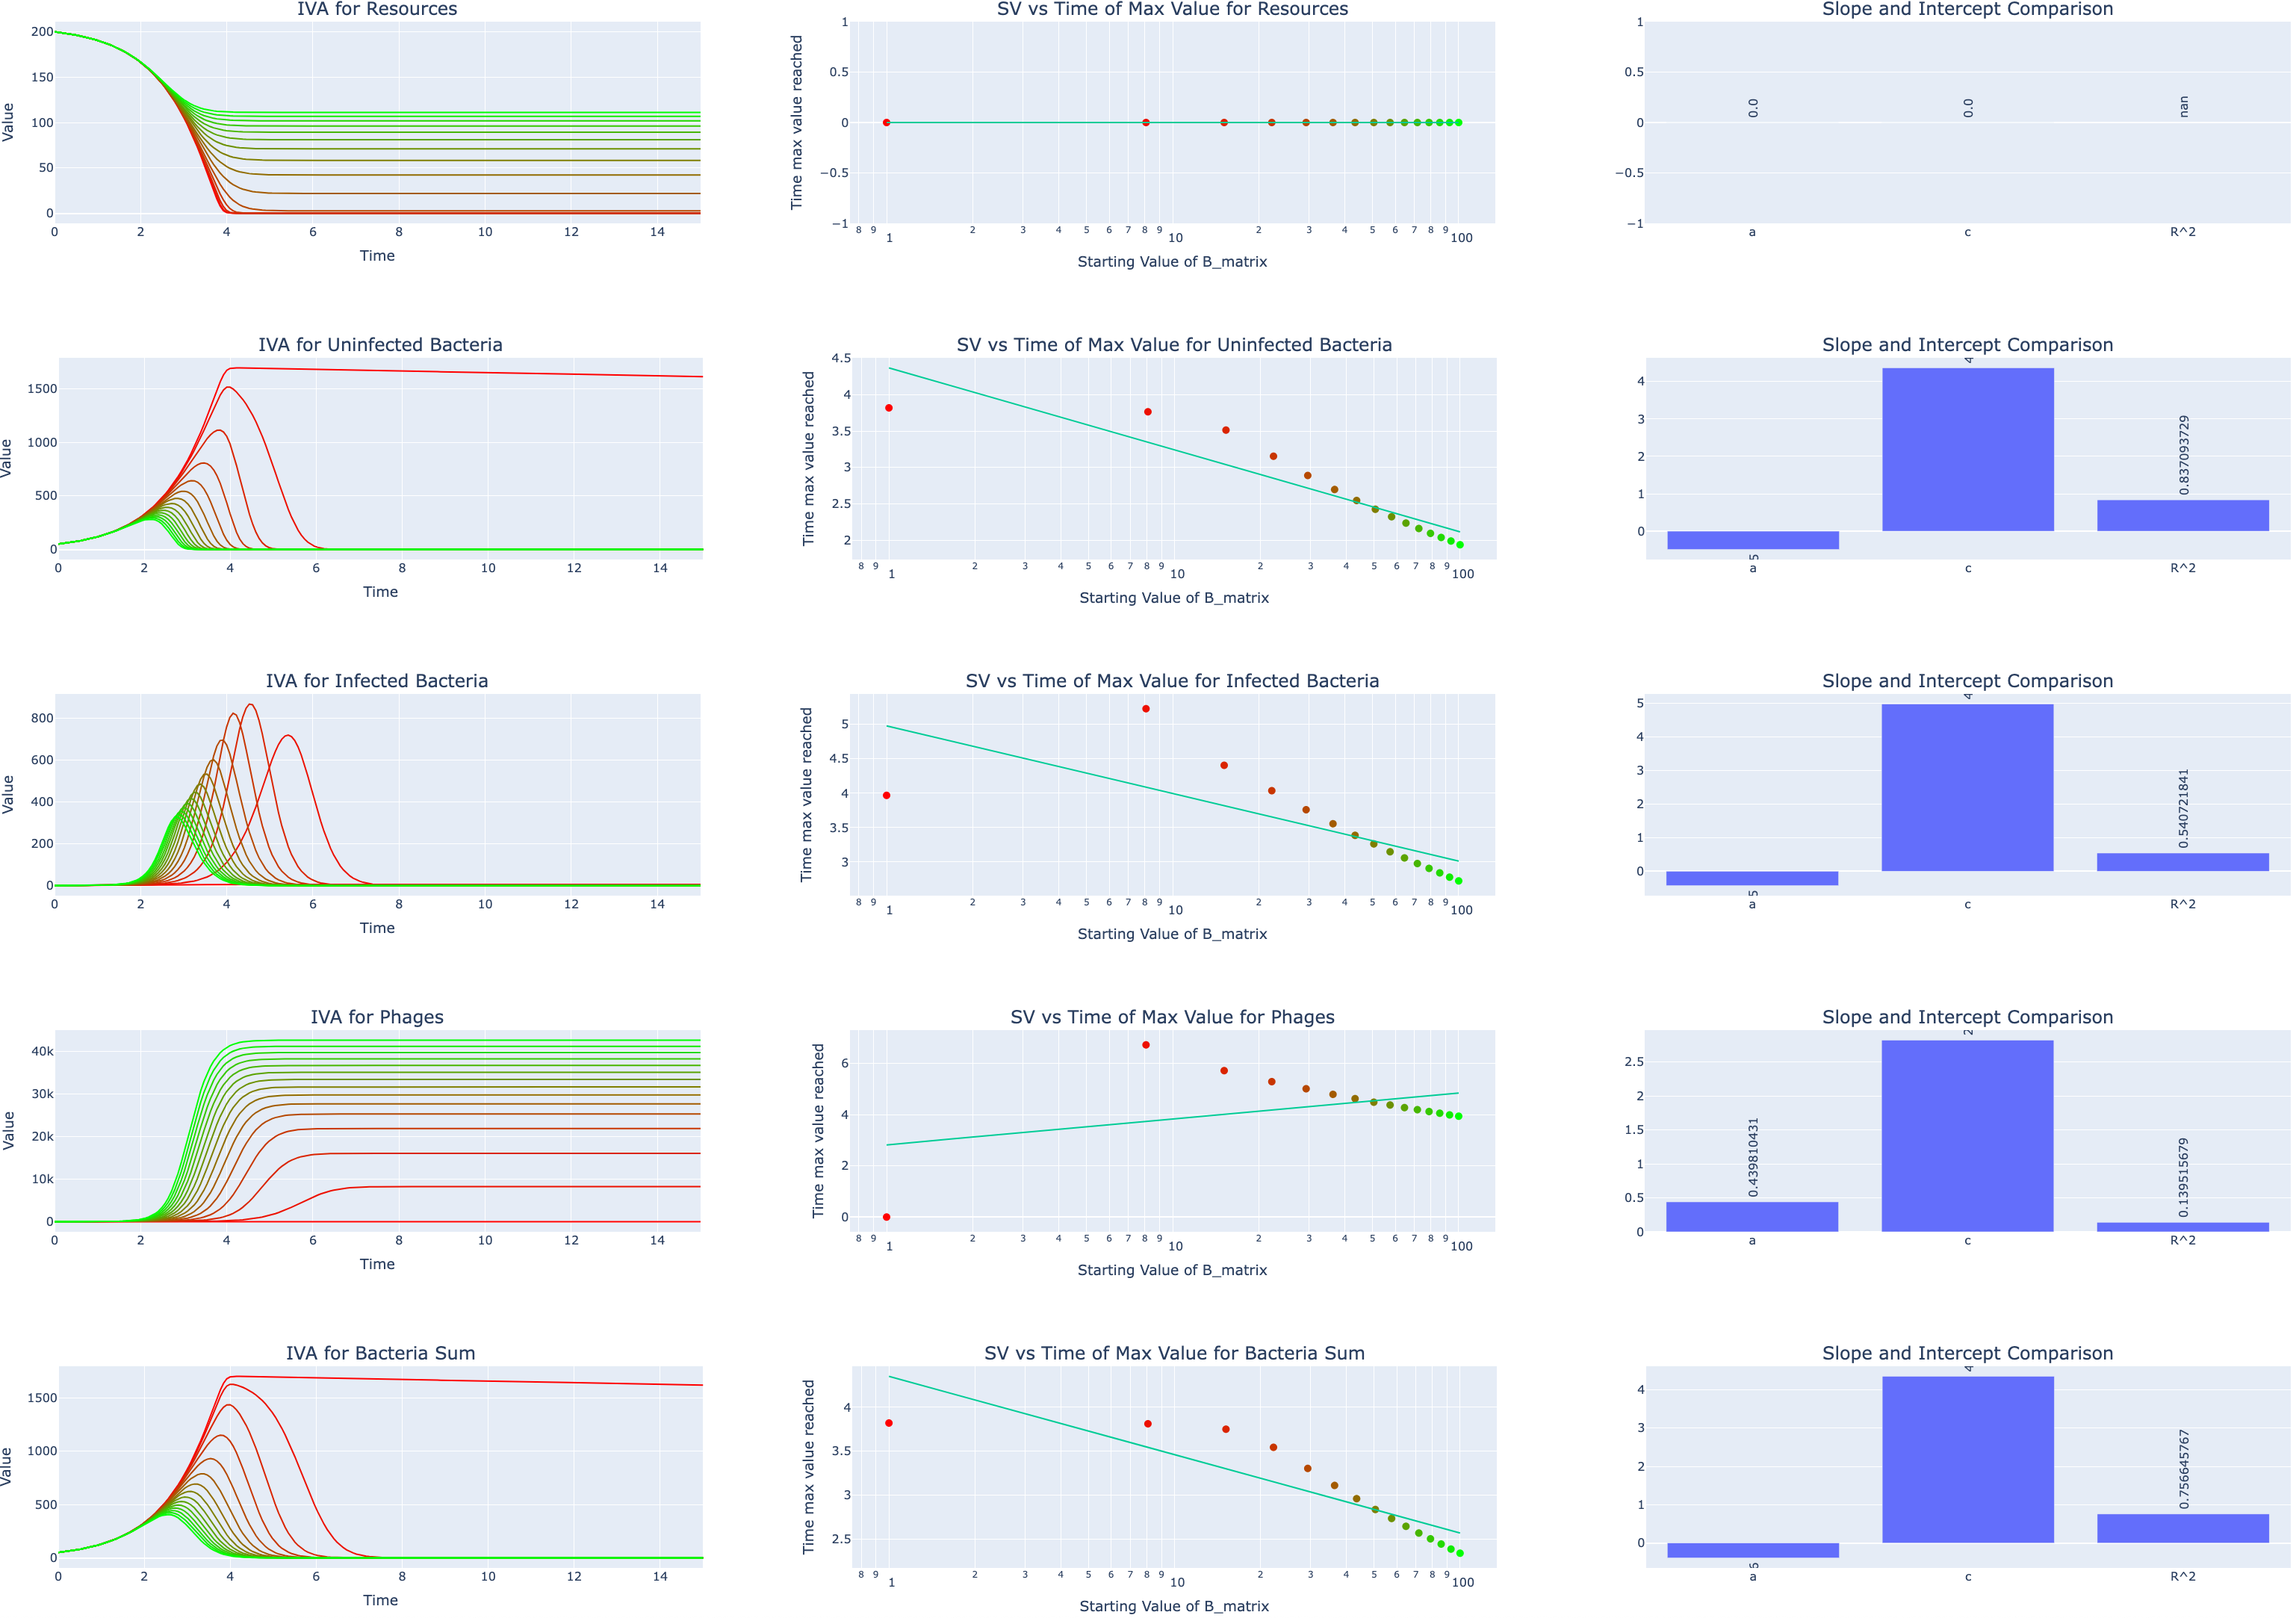
\includegraphics[width=1\textwidth]{Plots/Created/IVA/IVA_Table/beta.png}
    \centering
    \caption{
        Changing $\beta$ values. 
    }
    \label{fig:created:IVA_IVAtable_beta}
\end{figure}
